% Named preprint variant. Identical content to main.tex; differs only in the tmlr
% option ([preprint] prints the byline) and in switching on the camera-ready text.
% Build with: bash scripts/build_paper.sh main_preprint
% Do NOT submit this variant to TMLR, whose review is double-blind; submit main.pdf.
% TS-AgentBench manuscript.
%
% Target: Transactions on Machine Learning Research (TMLR).
%
% Why TMLR rather than a conference or Frontiers. TMLR's two acceptance criteria are
% (i) are the claims supported by accurate, convincing and clear evidence, and (ii)
% would some individuals in TMLR's audience be interested in the findings. There is
% explicitly no novelty or significance bar, and no page limit. That is the right venue
% for a measurement paper whose central result is partly negative and whose value is in
% the rigour of the measurement rather than in a new state of the art. The Frontiers
% variant of this manuscript is preserved at main_frontiers.tex; it uses the same
% section files, so both stay in sync.
%
% Style files (tmlr.sty, tmlr.bst, fancyhdr.sty) are from
% https://github.com/JmlrOrg/tmlr-style-file and are vendored alongside this file.
%   \usepackage{tmlr}             -> anonymous, for submission   (current)
%   \usepackage[preprint]{tmlr}   -> named, for arXiv
%   \usepackage[accepted]{tmlr}   -> camera-ready
%
% Build:
%   python scripts/make_paper_assets.py --run latest   # regenerate all numbers
%   latexmk -pdf main.tex
%
% INTEGRITY RULE: this manuscript contains no hardcoded experimental numbers.
% Every table is \input from tables/, every figure from figures/, and every number
% quoted inline is a macro defined in generated/macros.tex. All three are written by
% scripts/make_paper_assets.py from results/. If the experiment is rerun, the paper
% re-renders; the text cannot silently disagree with the data.

\documentclass{article}

\usepackage[preprint]{tmlr}

\usepackage[utf8]{inputenc}
\usepackage[T1]{fontenc}
\usepackage{amsmath,amssymb}
\usepackage{booktabs}
\usepackage{graphicx}
\usepackage{xcolor}
\usepackage{caption}
\usepackage{subcaption}
\usepackage{microtype}
\usepackage{url}

\graphicspath{{figures/}}

% Auto-generated numbers. Regenerate with scripts/make_paper_assets.py.
\IfFileExists{generated/macros.tex}{% Auto-generated by scripts/make_paper_assets.py. Do not edit by hand.
% Every number quoted in the manuscript prose is defined here, so the text
% cannot disagree with the experiment that produced it.
\newcommand{\runid}{main-20260918-233847-3fa46848}
\newcommand{\ntestinstances}{3284}
\newcommand{\nseries}{578}
\newcommand{\acceptmase}{1.0090}
\newcommand{\oraclemase}{0.7197}
\newcommand{\realizablemase}{1.0285}
\newcommand{\shouldcorrectrate}{59.2}
\newcommand{\maseAlwaysCorrect}{1.0978}
\newcommand{\regretAlwaysCorrect}{0.378}
\newcommand{\rateAlwaysCorrect}{100.0}
\newcommand{\helpedAlwaysCorrect}{26.4}
\newcommand{\harmedAlwaysCorrect}{29.2}
\newcommand{\deltaAlwaysCorrect}{8.80}
\newcommand{\maseBestFixed}{1.0981}
\newcommand{\regretBestFixed}{0.378}
\newcommand{\rateBestFixed}{90.3}
\newcommand{\helpedBestFixed}{29.3}
\newcommand{\harmedBestFixed}{32.3}
\newcommand{\deltaBestFixed}{8.83}
\newcommand{\maseNeverCorrect}{1.0090}
\newcommand{\regretNeverCorrect}{0.289}
\newcommand{\rateNeverCorrect}{0.0}
\newcommand{\helpedNeverCorrect}{??}
\newcommand{\harmedNeverCorrect}{??}
\newcommand{\deltaNeverCorrect}{0.00}
\newcommand{\maseRandomCorrect}{1.0365}
\newcommand{\regretRandomCorrect}{0.317}
\newcommand{\rateRandomCorrect}{21.0}
\newcommand{\helpedRandomCorrect}{29.9}
\newcommand{\harmedRandomCorrect}{43.6}
\newcommand{\deltaRandomCorrect}{2.72}
\newcommand{\maseRgc}{1.0132}
\newcommand{\regretRgc}{0.294}
\newcommand{\rateRgc}{20.0}
\newcommand{\helpedRgc}{51.0}
\newcommand{\harmedRgc}{39.9}
\newcommand{\deltaRgc}{0.42}
\newcommand{\maseThresholdSingle}{1.0701}
\newcommand{\regretThresholdSingle}{0.350}
\newcommand{\rateThresholdSingle}{29.0}
\newcommand{\helpedThresholdSingle}{18.8}
\newcommand{\harmedThresholdSingle}{26.8}
\newcommand{\deltaThresholdSingle}{6.05}
\newcommand{\verdictHOne}{not supported}
\newcommand{\statHOne}{0.421}
\newcommand{\verdictHTwo}{supported}
\newcommand{\statHTwo}{2.000}
\newcommand{\verdictHThree}{supported}
\newcommand{\statHThree}{0.793}
\newcommand{\verdictHFour}{supported}
\newcommand{\statHFour}{0.088}
\newcommand{\verdictHFive}{supported}
\newcommand{\statHFive}{0.220}
\newcommand{\verdictHSix}{supported}
\newcommand{\statHSix}{0.023}
\newcommand{\verdictHSeven}{supported}
\newcommand{\statHSeven}{0.094}
\newcommand{\triageauroc}{0.793}
\newcommand{\triagebaserate}{20.0}
\newcommand{\triageprecisionPFive}{76.2}
\newcommand{\triagerecallPFive}{19.0}
\newcommand{\triageliftPFive}{3.81}
\newcommand{\triageprecisionPOneZero}{66.5}
\newcommand{\triagerecallPOneZero}{33.2}
\newcommand{\triageliftPOneZero}{3.32}
\newcommand{\triageprecisionPTwoZero}{51.1}
\newcommand{\triagerecallPTwoZero}{51.0}
\newcommand{\triageliftPTwoZero}{2.55}
\newcommand{\triageprecisionPThreeZero}{42.4}
\newcommand{\triagerecallPThreeZero}{63.6}
\newcommand{\triageliftPThreeZero}{2.12}
\newcommand{\triageprecisionPFiveZero}{32.2}
\newcommand{\triagerecallPFiveZero}{80.5}
\newcommand{\triageliftPFiveZero}{1.61}
\newcommand{\maseAlwaysCorrectVsNeverPct}{8.13}
\newcommand{\maseAlwaysCorrectVsNeverCIlo}{2.73}
\newcommand{\maseAlwaysCorrectVsNeverCIhi}{15.99}
\newcommand{\maseAlwaysCorrectVsNeverWinRate}{45.8}
\newcommand{\maseAlwaysCorrectVsNeverSig}{yes}
\newcommand{\maseAlwaysCorrectVsNeverAbs}{8.13}
\newcommand{\maseAlwaysCorrectVsNeverAbsCIlo}{2.73}
\newcommand{\maseAlwaysCorrectVsNeverAbsCIhi}{15.99}
\newcommand{\maseAlwaysEnsembleVsNeverPct}{-4.69}
\newcommand{\maseAlwaysEnsembleVsNeverCIlo}{-11.75}
\newcommand{\maseAlwaysEnsembleVsNeverCIhi}{0.60}
\newcommand{\maseAlwaysEnsembleVsNeverWinRate}{60.0}
\newcommand{\maseAlwaysEnsembleVsNeverSig}{no}
\newcommand{\maseAlwaysEnsembleVsNeverAbs}{4.69}
\newcommand{\maseAlwaysEnsembleVsNeverAbsCIlo}{0.60}
\newcommand{\maseAlwaysEnsembleVsNeverAbsCIhi}{11.75}
\newcommand{\maseBestFixedVsNeverPct}{8.16}
\newcommand{\maseBestFixedVsNeverCIlo}{2.76}
\newcommand{\maseBestFixedVsNeverCIhi}{16.05}
\newcommand{\maseBestFixedVsNeverWinRate}{45.8}
\newcommand{\maseBestFixedVsNeverSig}{yes}
\newcommand{\maseBestFixedVsNeverAbs}{8.16}
\newcommand{\maseBestFixedVsNeverAbsCIlo}{2.76}
\newcommand{\maseBestFixedVsNeverAbsCIhi}{16.05}
\newcommand{\maseNeverCorrectVsNeverPct}{0.00}
\newcommand{\maseNeverCorrectVsNeverCIlo}{0.00}
\newcommand{\maseNeverCorrectVsNeverCIhi}{0.00}
\newcommand{\maseNeverCorrectVsNeverWinRate}{50.0}
\newcommand{\maseNeverCorrectVsNeverSig}{no}
\newcommand{\maseNeverCorrectVsNeverAbs}{0.00}
\newcommand{\maseNeverCorrectVsNeverAbsCIlo}{0.00}
\newcommand{\maseNeverCorrectVsNeverAbsCIhi}{0.00}
\newcommand{\maseRandomCorrectVsNeverPct}{4.13}
\newcommand{\maseRandomCorrectVsNeverCIlo}{2.12}
\newcommand{\maseRandomCorrectVsNeverCIhi}{6.46}
\newcommand{\maseRandomCorrectVsNeverWinRate}{42.6}
\newcommand{\maseRandomCorrectVsNeverSig}{yes}
\newcommand{\maseRandomCorrectVsNeverAbs}{4.13}
\newcommand{\maseRandomCorrectVsNeverAbsCIlo}{2.12}
\newcommand{\maseRandomCorrectVsNeverAbsCIhi}{6.46}
\newcommand{\maseRgcCalibratedVsNeverPct}{-0.38}
\newcommand{\maseRgcCalibratedVsNeverCIlo}{-0.97}
\newcommand{\maseRgcCalibratedVsNeverCIhi}{0.04}
\newcommand{\maseRgcCalibratedVsNeverWinRate}{50.2}
\newcommand{\maseRgcCalibratedVsNeverSig}{no}
\newcommand{\maseRgcCalibratedVsNeverAbs}{0.38}
\newcommand{\maseRgcCalibratedVsNeverAbsCIlo}{0.04}
\newcommand{\maseRgcCalibratedVsNeverAbsCIhi}{0.97}
\newcommand{\crpsAlwaysCorrectVsNeverPct}{5.31}
\newcommand{\crpsAlwaysCorrectVsNeverCIlo}{-0.38}
\newcommand{\crpsAlwaysCorrectVsNeverCIhi}{12.96}
\newcommand{\crpsAlwaysCorrectVsNeverWinRate}{54.8}
\newcommand{\crpsAlwaysCorrectVsNeverSig}{no}
\newcommand{\crpsAlwaysCorrectVsNeverAbs}{5.31}
\newcommand{\crpsAlwaysCorrectVsNeverAbsCIlo}{0.38}
\newcommand{\crpsAlwaysCorrectVsNeverAbsCIhi}{12.96}
\newcommand{\crpsAlwaysEnsembleVsNeverPct}{-13.07}
\newcommand{\crpsAlwaysEnsembleVsNeverCIlo}{-22.85}
\newcommand{\crpsAlwaysEnsembleVsNeverCIhi}{-7.27}
\newcommand{\crpsAlwaysEnsembleVsNeverWinRate}{65.4}
\newcommand{\crpsAlwaysEnsembleVsNeverSig}{yes}
\newcommand{\crpsAlwaysEnsembleVsNeverAbs}{13.07}
\newcommand{\crpsAlwaysEnsembleVsNeverAbsCIlo}{7.27}
\newcommand{\crpsAlwaysEnsembleVsNeverAbsCIhi}{22.85}
\newcommand{\crpsBestFixedVsNeverPct}{5.43}
\newcommand{\crpsBestFixedVsNeverCIlo}{-0.25}
\newcommand{\crpsBestFixedVsNeverCIhi}{13.05}
\newcommand{\crpsBestFixedVsNeverWinRate}{53.5}
\newcommand{\crpsBestFixedVsNeverSig}{no}
\newcommand{\crpsBestFixedVsNeverAbs}{5.43}
\newcommand{\crpsBestFixedVsNeverAbsCIlo}{0.25}
\newcommand{\crpsBestFixedVsNeverAbsCIhi}{13.05}
\newcommand{\crpsNeverCorrectVsNeverPct}{0.00}
\newcommand{\crpsNeverCorrectVsNeverCIlo}{0.00}
\newcommand{\crpsNeverCorrectVsNeverCIhi}{0.00}
\newcommand{\crpsNeverCorrectVsNeverWinRate}{50.0}
\newcommand{\crpsNeverCorrectVsNeverSig}{no}
\newcommand{\crpsNeverCorrectVsNeverAbs}{0.00}
\newcommand{\crpsNeverCorrectVsNeverAbsCIlo}{0.00}
\newcommand{\crpsNeverCorrectVsNeverAbsCIhi}{0.00}
\newcommand{\crpsRandomCorrectVsNeverPct}{4.25}
\newcommand{\crpsRandomCorrectVsNeverCIlo}{2.24}
\newcommand{\crpsRandomCorrectVsNeverCIhi}{6.58}
\newcommand{\crpsRandomCorrectVsNeverWinRate}{42.1}
\newcommand{\crpsRandomCorrectVsNeverSig}{yes}
\newcommand{\crpsRandomCorrectVsNeverAbs}{4.25}
\newcommand{\crpsRandomCorrectVsNeverAbsCIlo}{2.24}
\newcommand{\crpsRandomCorrectVsNeverAbsCIhi}{6.58}
\newcommand{\crpsRgcCalibratedVsNeverPct}{-4.04}
\newcommand{\crpsRgcCalibratedVsNeverCIlo}{-14.47}
\newcommand{\crpsRgcCalibratedVsNeverCIhi}{2.87}
\newcommand{\crpsRgcCalibratedVsNeverWinRate}{61.0}
\newcommand{\crpsRgcCalibratedVsNeverSig}{no}
\newcommand{\crpsRgcCalibratedVsNeverAbs}{4.04}
\newcommand{\crpsRgcCalibratedVsNeverAbsCIlo}{2.87}
\newcommand{\crpsRgcCalibratedVsNeverAbsCIhi}{14.47}
\newcommand{\llmMaseAlwaysCorrectPct}{5.73}
\newcommand{\llmMaseAlwaysCorrectCIlo}{-0.48}
\newcommand{\llmMaseAlwaysCorrectCIhi}{14.43}
\newcommand{\llmMaseAlwaysCorrectWinRate}{47.1}
\newcommand{\llmMaseAlwaysCorrectNseries}{578}
\newcommand{\llmMaseAlwaysCorrectAbs}{5.73}
\newcommand{\llmMaseAlwaysCorrectAbsCIlo}{0.48}
\newcommand{\llmMaseAlwaysCorrectAbsCIhi}{14.43}
\newcommand{\llmMaseAlwaysEnsemblePct}{-5.73}
\newcommand{\llmMaseAlwaysEnsembleCIlo}{-9.54}
\newcommand{\llmMaseAlwaysEnsembleCIhi}{-1.99}
\newcommand{\llmMaseAlwaysEnsembleWinRate}{53.9}
\newcommand{\llmMaseAlwaysEnsembleNseries}{578}
\newcommand{\llmMaseAlwaysEnsembleAbs}{5.73}
\newcommand{\llmMaseAlwaysEnsembleAbsCIlo}{1.99}
\newcommand{\llmMaseAlwaysEnsembleAbsCIhi}{9.54}
\newcommand{\llmMaseLlmCritiqueGatePct}{7.50}
\newcommand{\llmMaseLlmCritiqueGateCIlo}{2.73}
\newcommand{\llmMaseLlmCritiqueGateCIhi}{12.89}
\newcommand{\llmMaseLlmCritiqueGateWinRate}{42.8}
\newcommand{\llmMaseLlmCritiqueGateNseries}{578}
\newcommand{\llmMaseLlmCritiqueGateAbs}{7.50}
\newcommand{\llmMaseLlmCritiqueGateAbsCIlo}{2.73}
\newcommand{\llmMaseLlmCritiqueGateAbsCIhi}{12.89}
\newcommand{\llmMaseLlmSinglePct}{8.37}
\newcommand{\llmMaseLlmSingleCIlo}{3.29}
\newcommand{\llmMaseLlmSingleCIhi}{13.94}
\newcommand{\llmMaseLlmSingleWinRate}{42.2}
\newcommand{\llmMaseLlmSingleNseries}{578}
\newcommand{\llmMaseLlmSingleAbs}{8.37}
\newcommand{\llmMaseLlmSingleAbsCIlo}{3.29}
\newcommand{\llmMaseLlmSingleAbsCIhi}{13.94}
\newcommand{\llmMaseNeverCorrectPct}{0.00}
\newcommand{\llmMaseNeverCorrectCIlo}{0.00}
\newcommand{\llmMaseNeverCorrectCIhi}{0.00}
\newcommand{\llmMaseNeverCorrectWinRate}{50.0}
\newcommand{\llmMaseNeverCorrectNseries}{578}
\newcommand{\llmMaseNeverCorrectAbs}{0.00}
\newcommand{\llmMaseNeverCorrectAbsCIlo}{0.00}
\newcommand{\llmMaseNeverCorrectAbsCIhi}{0.00}
\newcommand{\llmMaseRgcCalibratedPct}{-0.19}
\newcommand{\llmMaseRgcCalibratedCIlo}{-0.72}
\newcommand{\llmMaseRgcCalibratedCIhi}{0.26}
\newcommand{\llmMaseRgcCalibratedWinRate}{50.3}
\newcommand{\llmMaseRgcCalibratedNseries}{578}
\newcommand{\llmMaseRgcCalibratedAbs}{0.19}
\newcommand{\llmMaseRgcCalibratedAbsCIlo}{0.26}
\newcommand{\llmMaseRgcCalibratedAbsCIhi}{0.72}
\newcommand{\llmMaseRgcLlmRouterPct}{4.87}
\newcommand{\llmMaseRgcLlmRouterCIlo}{0.95}
\newcommand{\llmMaseRgcLlmRouterCIhi}{10.06}
\newcommand{\llmMaseRgcLlmRouterWinRate}{47.5}
\newcommand{\llmMaseRgcLlmRouterNseries}{578}
\newcommand{\llmMaseRgcLlmRouterAbs}{4.87}
\newcommand{\llmMaseRgcLlmRouterAbsCIlo}{0.95}
\newcommand{\llmMaseRgcLlmRouterAbsCIhi}{10.06}
\newcommand{\llmCrpsAlwaysCorrectPct}{3.29}
\newcommand{\llmCrpsAlwaysCorrectCIlo}{-4.92}
\newcommand{\llmCrpsAlwaysCorrectCIhi}{13.64}
\newcommand{\llmCrpsAlwaysCorrectWinRate}{51.6}
\newcommand{\llmCrpsAlwaysCorrectNseries}{578}
\newcommand{\llmCrpsAlwaysCorrectAbs}{3.29}
\newcommand{\llmCrpsAlwaysCorrectAbsCIlo}{4.92}
\newcommand{\llmCrpsAlwaysCorrectAbsCIhi}{13.64}
\newcommand{\llmCrpsAlwaysEnsemblePct}{-10.59}
\newcommand{\llmCrpsAlwaysEnsembleCIlo}{-15.14}
\newcommand{\llmCrpsAlwaysEnsembleCIhi}{-6.70}
\newcommand{\llmCrpsAlwaysEnsembleWinRate}{53.8}
\newcommand{\llmCrpsAlwaysEnsembleNseries}{578}
\newcommand{\llmCrpsAlwaysEnsembleAbs}{10.59}
\newcommand{\llmCrpsAlwaysEnsembleAbsCIlo}{6.70}
\newcommand{\llmCrpsAlwaysEnsembleAbsCIhi}{15.14}
\newcommand{\llmCrpsLlmCritiqueGatePct}{8.13}
\newcommand{\llmCrpsLlmCritiqueGateCIlo}{3.17}
\newcommand{\llmCrpsLlmCritiqueGateCIhi}{13.92}
\newcommand{\llmCrpsLlmCritiqueGateWinRate}{44.3}
\newcommand{\llmCrpsLlmCritiqueGateNseries}{578}
\newcommand{\llmCrpsLlmCritiqueGateAbs}{8.13}
\newcommand{\llmCrpsLlmCritiqueGateAbsCIlo}{3.17}
\newcommand{\llmCrpsLlmCritiqueGateAbsCIhi}{13.92}
\newcommand{\llmCrpsLlmSinglePct}{8.48}
\newcommand{\llmCrpsLlmSingleCIlo}{3.00}
\newcommand{\llmCrpsLlmSingleCIhi}{14.55}
\newcommand{\llmCrpsLlmSingleWinRate}{43.9}
\newcommand{\llmCrpsLlmSingleNseries}{578}
\newcommand{\llmCrpsLlmSingleAbs}{8.48}
\newcommand{\llmCrpsLlmSingleAbsCIlo}{3.00}
\newcommand{\llmCrpsLlmSingleAbsCIhi}{14.55}
\newcommand{\llmCrpsNeverCorrectPct}{0.00}
\newcommand{\llmCrpsNeverCorrectCIlo}{0.00}
\newcommand{\llmCrpsNeverCorrectCIhi}{0.00}
\newcommand{\llmCrpsNeverCorrectWinRate}{50.0}
\newcommand{\llmCrpsNeverCorrectNseries}{578}
\newcommand{\llmCrpsNeverCorrectAbs}{0.00}
\newcommand{\llmCrpsNeverCorrectAbsCIlo}{0.00}
\newcommand{\llmCrpsNeverCorrectAbsCIhi}{0.00}
\newcommand{\llmCrpsRgcCalibratedPct}{-5.31}
\newcommand{\llmCrpsRgcCalibratedCIlo}{-9.36}
\newcommand{\llmCrpsRgcCalibratedCIhi}{-1.91}
\newcommand{\llmCrpsRgcCalibratedWinRate}{53.5}
\newcommand{\llmCrpsRgcCalibratedNseries}{578}
\newcommand{\llmCrpsRgcCalibratedAbs}{5.31}
\newcommand{\llmCrpsRgcCalibratedAbsCIlo}{1.91}
\newcommand{\llmCrpsRgcCalibratedAbsCIhi}{9.36}
\newcommand{\llmCrpsRgcLlmRouterPct}{3.63}
\newcommand{\llmCrpsRgcLlmRouterCIlo}{0.48}
\newcommand{\llmCrpsRgcLlmRouterCIhi}{8.04}
\newcommand{\llmCrpsRgcLlmRouterWinRate}{48.7}
\newcommand{\llmCrpsRgcLlmRouterNseries}{578}
\newcommand{\llmCrpsRgcLlmRouterAbs}{3.63}
\newcommand{\llmCrpsRgcLlmRouterAbsCIlo}{0.48}
\newcommand{\llmCrpsRgcLlmRouterAbsCIhi}{8.04}
\newcommand{\rateLlmCritiqueGate}{69.9}
\newcommand{\helpedLlmCritiqueGateLlm}{29.0}
\newcommand{\harmedLlmCritiqueGateLlm}{49.5}
\newcommand{\rateLlmSingle}{68.7}
\newcommand{\helpedLlmSingleLlm}{27.7}
\newcommand{\harmedLlmSingleLlm}{50.4}
\newcommand{\rateRgcLlmRouter}{14.4}
\newcommand{\helpedRgcLlmRouterLlm}{28.9}
\newcommand{\harmedRgcLlmRouterLlm}{63.9}
\newcommand{\discrimAurocCritique}{0.532}
\newcommand{\discrimAurocSingle}{0.522}
\newcommand{\discrimAurocDelta}{0.010}
\newcommand{\discrimJaccard}{82}
\newcommand{\discrimBaseRate}{59.7}
\newcommand{\discrimPrecisionCritique}{61.9}
\newcommand{\discrimPrecisionRandom}{59.9}
\newcommand{\discrimN}{578}
\newcommand{\discrimAurocArithmetic}{0.760}
\newcommand{\discrimAurocLlmConfidence}{0.529}
\newcommand{\discrimBalaccCritique}{0.532}
\newcommand{\discrimBalaccArithmetic}{0.672}
\newcommand{\discrimContinuousGap}{0.231}
\newcommand{\discrimMatchedGap}{0.140}
\newcommand{\discrimArithmeticAdvantage}{0.229}
\newcommand{\actionChoiceSinglePct}{3.55}
\newcommand{\actionChoiceSingleCIlo}{-4.07}
\newcommand{\actionChoiceSingleCIhi}{12.11}
\newcommand{\actionChoiceSingleN}{361}
\newcommand{\actionChoiceSingleGap}{72.5}
\newcommand{\actionChoiceSingleGapCIlo}{56.6}
\newcommand{\actionChoiceSingleGapCIhi}{91.7}
\newcommand{\actionChoiceSingleHeadroom}{-8.9}
\newcommand{\actionChoiceSingleHeadroomCIlo}{-30.6}
\newcommand{\actionChoiceSingleHeadroomCIhi}{10.2}
\newcommand{\actionChoiceChosen}{1.119}
\newcommand{\actionChoiceBest}{0.649}
\newcommand{\actionChoiceRandom}{1.081}
\newcommand{\actionChoiceWorst}{2.061}
\newcommand{\actionChoiceCritiquePct}{2.13}
\newcommand{\actionChoiceCritiqueCIlo}{-5.17}
\newcommand{\actionChoiceCritiqueCIhi}{10.66}
\newcommand{\actionChoiceCritiqueN}{367}
\newcommand{\actionChoiceCritiqueGap}{73.9}
\newcommand{\actionChoiceCritiqueGapCIlo}{57.4}
\newcommand{\actionChoiceCritiqueGapCIhi}{93.4}
\newcommand{\actionChoiceCritiqueHeadroom}{-5.2}
\newcommand{\actionChoiceCritiqueHeadroomCIlo}{-25.4}
\newcommand{\actionChoiceCritiqueHeadroomCIhi}{12.7}
\newcommand{\actionChoiceRouterPct}{28.31}
\newcommand{\actionChoiceRouterCIlo}{-0.99}
\newcommand{\actionChoiceRouterCIhi}{65.84}
\newcommand{\actionChoiceRouterN}{80}
\newcommand{\actionChoiceRouterGap}{178.4}
\newcommand{\actionChoiceRouterGapCIlo}{97.5}
\newcommand{\actionChoiceRouterGapCIhi}{303.8}
\newcommand{\actionChoiceRouterHeadroom}{-52.5}
\newcommand{\actionChoiceRouterHeadroomCIlo}{-110.0}
\newcommand{\actionChoiceRouterHeadroomCIhi}{2.1}
\newcommand{\reasonMaseSinglePct}{5.52}
\newcommand{\reasonMaseSingleCIlo}{-2.92}
\newcommand{\reasonMaseSingleCIhi}{14.61}
\newcommand{\reasonSeries}{60}
\newcommand{\reasonMaseCritiquePct}{5.62}
\newcommand{\reasonMaseCritiqueCIlo}{-3.77}
\newcommand{\reasonMaseCritiqueCIhi}{15.32}
\newcommand{\reasonCrpsSinglePct}{6.49}
\newcommand{\reasonCrpsSingleCIlo}{-2.30}
\newcommand{\reasonCrpsSingleCIhi}{15.67}
\newcommand{\reasonCrpsCritiquePct}{6.81}
\newcommand{\reasonCrpsCritiqueCIlo}{-1.72}
\newcommand{\reasonCrpsCritiqueCIhi}{15.52}
\newcommand{\reasonRateSingle}{90}
\newcommand{\reasonRateCritique}{78}
\newcommand{\fewshotMaseSinglePct}{6.65}
\newcommand{\fewshotMaseSingleCIlo}{-1.25}
\newcommand{\fewshotMaseSingleCIhi}{15.77}
\newcommand{\fewshotSeries}{60}
\newcommand{\fewshotMaseCritiquePct}{28.85}
\newcommand{\fewshotMaseCritiqueCIlo}{-0.49}
\newcommand{\fewshotMaseCritiqueCIhi}{80.30}
\newcommand{\fewshotCrpsSinglePct}{8.33}
\newcommand{\fewshotCrpsSingleCIlo}{0.49}
\newcommand{\fewshotCrpsSingleCIhi}{16.66}
\newcommand{\fewshotCrpsCritiquePct}{23.09}
\newcommand{\fewshotCrpsCritiqueCIlo}{1.96}
\newcommand{\fewshotCrpsCritiqueCIhi}{58.52}
\newcommand{\fewshotRateSingle}{67}
\newcommand{\fewshotRateCritique}{67}
\newcommand{\zeroshotMaseSinglePct}{8.45}
\newcommand{\zeroshotMaseSingleCIlo}{3.00}
\newcommand{\zeroshotMaseSingleCIhi}{14.72}
\newcommand{\zeroshotSeries}{60}
\newcommand{\zeroshotMaseCritiquePct}{9.19}
\newcommand{\zeroshotMaseCritiqueCIlo}{1.69}
\newcommand{\zeroshotMaseCritiqueCIhi}{17.60}
\newcommand{\zeroshotCrpsSinglePct}{8.73}
\newcommand{\zeroshotCrpsSingleCIlo}{2.75}
\newcommand{\zeroshotCrpsSingleCIhi}{15.62}
\newcommand{\zeroshotCrpsCritiquePct}{11.06}
\newcommand{\zeroshotCrpsCritiqueCIlo}{4.34}
\newcommand{\zeroshotCrpsCritiqueCIhi}{18.85}
\newcommand{\zeroshotRateSingle}{68}
\newcommand{\zeroshotRateCritique}{77}
\newcommand{\reasonAurocCritique}{0.493}
\newcommand{\reasonAurocSingle}{0.590}
\newcommand{\reasonAurocArithmetic}{0.774}
\newcommand{\reasonAurocDelta}{-0.097}
\newcommand{\reasonDiscrimN}{60}
\newcommand{\reasonHeadroomSingle}{40.0}
\newcommand{\reasonHeadroomSingleCIlo}{-0.8}
\newcommand{\reasonHeadroomSingleCIhi}{67.1}
\newcommand{\reasonGapSingle}{39.8}
\newcommand{\reasonChoiceSinglePct}{-15.96}
\newcommand{\reasonChoiceSingleCIlo}{-37.65}
\newcommand{\reasonChoiceSingleCIhi}{0.23}
\newcommand{\reasonHeadroomCritique}{32.0}
\newcommand{\reasonHeadroomCritiqueCIlo}{-5.8}
\newcommand{\reasonHeadroomCritiqueCIhi}{60.4}
\newcommand{\reasonGapCritique}{38.9}
\newcommand{\reasonChoiceCritiquePct}{-11.64}
\newcommand{\reasonChoiceCritiqueCIlo}{-26.45}
\newcommand{\reasonChoiceCritiqueCIhi}{1.77}
\newcommand{\calLlmEce}{0.325}
\newcommand{\calLlmBrier}{0.315}
\newcommand{\calLlmAurc}{0.159}
\newcommand{\calLlmMeanRisk}{0.544}
\newcommand{\calEstEce}{0.050}
\newcommand{\calEstBrier}{0.140}
\newcommand{\calEstAurc}{0.088}
\newcommand{\calConstBrier}{0.171}
\newcommand{\calConstAurc}{0.229}
\newcommand{\calBaseRate}{22.0}
\newcommand{\calN}{578}
\newcommand{\calEceDiff}{0.220}
\newcommand{\calEceDiffCIlo}{0.188}
\newcommand{\calEceDiffCIhi}{0.252}
\newcommand{\ablFull}{0.00}
\newcommand{\ablFullRate}{20.0}
\newcommand{\ablFullCompute}{0.79}
\newcommand{\ablFullSeries}{0.00}
\newcommand{\ablFullSeriesCIlo}{0.00}
\newcommand{\ablFullSeriesCIhi}{0.00}
\newcommand{\ablNoSelfCritique}{0.18}
\newcommand{\ablNoSelfCritiqueRate}{24.1}
\newcommand{\ablNoSelfCritiqueCompute}{2.38}
\newcommand{\ablNoSelfCritiqueSeries}{0.12}
\newcommand{\ablNoSelfCritiqueSeriesCIlo}{-2.75}
\newcommand{\ablNoSelfCritiqueSeriesCIhi}{2.09}
\newcommand{\ablNoUncertainty}{-1.45}
\newcommand{\ablNoUncertaintyRate}{21.3}
\newcommand{\ablNoUncertaintyCompute}{0.83}
\newcommand{\ablNoUncertaintySeries}{-1.36}
\newcommand{\ablNoUncertaintySeriesCIlo}{-3.97}
\newcommand{\ablNoUncertaintySeriesCIhi}{0.10}
\newcommand{\ablNoModelDisagreement}{-0.14}
\newcommand{\ablNoModelDisagreementRate}{20.2}
\newcommand{\ablNoModelDisagreementCompute}{0.80}
\newcommand{\ablNoModelDisagreementSeries}{-0.11}
\newcommand{\ablNoModelDisagreementSeriesCIlo}{-0.41}
\newcommand{\ablNoModelDisagreementSeriesCIhi}{0.16}
\newcommand{\ablNoChangepoint}{-1.02}
\newcommand{\ablNoChangepointRate}{20.5}
\newcommand{\ablNoChangepointCompute}{0.82}
\newcommand{\ablNoChangepointSeries}{-0.98}
\newcommand{\ablNoChangepointSeriesCIlo}{-3.52}
\newcommand{\ablNoChangepointSeriesCIhi}{0.42}
\newcommand{\ablNoAnomaly}{-0.24}
\newcommand{\ablNoAnomalyRate}{20.1}
\newcommand{\ablNoAnomalyCompute}{0.78}
\newcommand{\ablNoAnomalySeries}{-0.18}
\newcommand{\ablNoAnomalySeriesCIlo}{-3.01}
\newcommand{\ablNoAnomalySeriesCIhi}{1.67}
\newcommand{\ablNoAdaptiveTools}{0.18}
\newcommand{\ablNoAdaptiveToolsRate}{24.1}
\newcommand{\ablNoAdaptiveToolsCompute}{2.38}
\newcommand{\ablNoAdaptiveToolsSeries}{0.12}
\newcommand{\ablNoAdaptiveToolsSeriesCIlo}{-2.75}
\newcommand{\ablNoAdaptiveToolsSeriesCIhi}{2.09}
\newcommand{\ablNoBacktesting}{2.68}
\newcommand{\ablNoBacktestingRate}{27.6}
\newcommand{\ablNoBacktestingCompute}{0.83}
\newcommand{\ablNoBacktestingSeries}{4.41}
\newcommand{\ablNoBacktestingSeriesCIlo}{0.92}
\newcommand{\ablNoBacktestingSeriesCIhi}{7.41}
\newcommand{\ablNoCorrectionLoop}{-0.42}
\newcommand{\ablNoCorrectionLoopRate}{0.0}
\newcommand{\ablNoCorrectionLoopCompute}{0.00}
\newcommand{\ablNoCorrectionLoopSeries}{-0.13}
\newcommand{\ablNoCorrectionLoopSeriesCIlo}{-3.02}
\newcommand{\ablNoCorrectionLoopSeriesCIhi}{1.84}
\newcommand{\robComparisons}{48}
\newcommand{\robImprovements}{0}
\newcommand{\robDegradations}{4}
\newcommand{\robHTwoTested}{48}
\newcommand{\robHTwoRaw}{10}
\newcommand{\robHTwoSurviving}{2}
\newcommand{\robOracleMild}{31.9}
\newcommand{\robOracleSevere}{32.9}
\newcommand{\robShouldCorrectMild}{65.8}
\newcommand{\robShouldCorrectSevere}{68.6}
\newcommand{\robSeverityMild}{0.25}
\newcommand{\robSeveritySevere}{1.00}
\newcommand{\robHTwoPolicies}{always correct}
\newcommand{\robHTwoAxes}{artificial anomalies, gaussian noise}
\newcommand{\robHTwoSeverity}{0.25}
\newcommand{\fbReading}{B}
\newcommand{\fbSingleFactorOk}{yes}
\newcommand{\fbAlwaysCorrectAdaptivePct}{8.13}
\newcommand{\fbAlwaysCorrectAdaptiveCIlo}{2.73}
\newcommand{\fbAlwaysCorrectAdaptiveCIhi}{15.99}
\newcommand{\fbAlwaysCorrectFixedPct}{10.59}
\newcommand{\fbAlwaysCorrectFixedCIlo}{1.21}
\newcommand{\fbAlwaysCorrectFixedCIhi}{27.56}
\newcommand{\fbBestFixedAdaptivePct}{8.16}
\newcommand{\fbBestFixedAdaptiveCIlo}{2.76}
\newcommand{\fbBestFixedAdaptiveCIhi}{16.05}
\newcommand{\fbBestFixedFixedPct}{10.52}
\newcommand{\fbBestFixedFixedCIlo}{1.15}
\newcommand{\fbBestFixedFixedCIhi}{27.49}
\newcommand{\fbLlmSingleAdaptivePct}{??}
\newcommand{\fbLlmSingleAdaptiveCIlo}{??}
\newcommand{\fbLlmSingleAdaptiveCIhi}{??}
\newcommand{\fbLlmSingleFixedPct}{-2.56}
\newcommand{\fbLlmSingleFixedCIlo}{-27.38}
\newcommand{\fbLlmSingleFixedCIhi}{14.44}
\newcommand{\fbRandomCorrectAdaptivePct}{2.72}
\newcommand{\fbRandomCorrectAdaptiveCIlo}{2.06}
\newcommand{\fbRandomCorrectAdaptiveCIhi}{3.46}
\newcommand{\fbRandomCorrectFixedPct}{3.59}
\newcommand{\fbRandomCorrectFixedCIlo}{2.88}
\newcommand{\fbRandomCorrectFixedCIhi}{4.40}
\newcommand{\fbRgcAdaptivePct}{0.14}
\newcommand{\fbRgcAdaptiveCIlo}{-1.84}
\newcommand{\fbRgcAdaptiveCIhi}{3.03}
\newcommand{\fbRgcFixedPct}{-0.49}
\newcommand{\fbRgcFixedCIlo}{-1.64}
\newcommand{\fbRgcFixedCIhi}{0.67}
\newcommand{\fbRgcCalibratedAdaptivePct}{??}
\newcommand{\fbRgcCalibratedAdaptiveCIlo}{??}
\newcommand{\fbRgcCalibratedAdaptiveCIhi}{??}
\newcommand{\fbRgcCalibratedFixedPct}{1.62}
\newcommand{\fbRgcCalibratedFixedCIlo}{-0.56}
\newcommand{\fbRgcCalibratedFixedCIhi}{4.20}
\newcommand{\fbThresholdSingleAdaptivePct}{5.48}
\newcommand{\fbThresholdSingleAdaptiveCIlo}{1.46}
\newcommand{\fbThresholdSingleAdaptiveCIhi}{10.88}
\newcommand{\fbThresholdSingleFixedPct}{3.95}
\newcommand{\fbThresholdSingleFixedCIlo}{0.53}
\newcommand{\fbThresholdSingleFixedCIhi}{9.29}
\newcommand{\rdMaseNseries}{420}
\newcommand{\rdMaseCanonical}{2.43}
\newcommand{\rdMaseCanonicalCIlo}{-0.50}
\newcommand{\rdMaseCanonicalCIhi}{5.33}
\newcommand{\rdMaseValMatched}{5.33}
\newcommand{\rdMaseValMatchedCIlo}{-3.20}
\newcommand{\rdMaseValMatchedCIhi}{19.19}
\newcommand{\rdMaseValAny}{4.45}
\newcommand{\rdMaseValAnyCIlo}{0.16}
\newcommand{\rdMaseValAnyCIhi}{9.95}
\newcommand{\rdMaseTestMatched}{-15.12}
\newcommand{\rdMaseTestMatchedCIlo}{-17.60}
\newcommand{\rdMaseTestMatchedCIhi}{-12.80}
\newcommand{\rdMaseTestAny}{-31.24}
\newcommand{\rdMaseTestAnyCIlo}{-33.46}
\newcommand{\rdMaseTestAnyCIhi}{-29.10}
\newcommand{\rdMaseRealTotal}{4.45}
\newcommand{\rdMaseRealTotalCIlo}{0.16}
\newcommand{\rdMaseRealTotalCIhi}{9.95}
\newcommand{\rdMaseRealFirst}{-2.90}
\newcommand{\rdMaseRealFirstCIlo}{-16.62}
\newcommand{\rdMaseRealFirstCIhi}{5.49}
\newcommand{\rdMaseRealRestrict}{0.88}
\newcommand{\rdMaseRealRestrictCIlo}{-5.13}
\newcommand{\rdMaseRealRestrictCIhi}{9.89}
\newcommand{\rdMaseCeilTotal}{-31.24}
\newcommand{\rdMaseCeilTotalCIlo}{-33.46}
\newcommand{\rdMaseCeilTotalCIhi}{-29.10}
\newcommand{\rdMaseCeilFirst}{17.55}
\newcommand{\rdMaseCeilFirstCIlo}{14.79}
\newcommand{\rdMaseCeilFirstCIhi}{20.50}
\newcommand{\rdMaseCeilRestrict}{16.12}
\newcommand{\rdMaseCeilRestrictCIlo}{14.49}
\newcommand{\rdMaseCeilRestrictCIhi}{17.87}
\newcommand{\rdMaseCeilTotalAbs}{31.24}
\newcommand{\rdMaseCurseShare}{114}
\newcommand{\rdCrpsNseries}{420}
\newcommand{\rdCrpsCanonical}{3.59}
\newcommand{\rdCrpsCanonicalCIlo}{0.03}
\newcommand{\rdCrpsCanonicalCIhi}{7.26}
\newcommand{\rdCrpsValMatched}{3.76}
\newcommand{\rdCrpsValMatchedCIlo}{-6.54}
\newcommand{\rdCrpsValMatchedCIhi}{20.33}
\newcommand{\rdCrpsValAny}{-0.80}
\newcommand{\rdCrpsValAnyCIlo}{-4.24}
\newcommand{\rdCrpsValAnyCIhi}{2.79}
\newcommand{\rdCrpsTestMatched}{-19.52}
\newcommand{\rdCrpsTestMatchedCIlo}{-22.05}
\newcommand{\rdCrpsTestMatchedCIhi}{-17.01}
\newcommand{\rdCrpsTestAny}{-33.42}
\newcommand{\rdCrpsTestAnyCIlo}{-35.77}
\newcommand{\rdCrpsTestAnyCIhi}{-31.11}
\newcommand{\rdCrpsRealTotal}{-0.80}
\newcommand{\rdCrpsRealTotalCIlo}{-4.24}
\newcommand{\rdCrpsRealTotalCIhi}{2.79}
\newcommand{\rdCrpsRealFirst}{-0.17}
\newcommand{\rdCrpsRealFirstCIlo}{-16.69}
\newcommand{\rdCrpsRealFirstCIhi}{10.45}
\newcommand{\rdCrpsRealRestrict}{4.56}
\newcommand{\rdCrpsRealRestrictCIlo}{-4.44}
\newcommand{\rdCrpsRealRestrictCIhi}{19.25}
\newcommand{\rdCrpsCeilTotal}{-33.42}
\newcommand{\rdCrpsCeilTotalCIlo}{-35.77}
\newcommand{\rdCrpsCeilTotalCIhi}{-31.11}
\newcommand{\rdCrpsCeilFirst}{23.11}
\newcommand{\rdCrpsCeilFirstCIlo}{19.67}
\newcommand{\rdCrpsCeilFirstCIhi}{26.83}
\newcommand{\rdCrpsCeilRestrict}{13.90}
\newcommand{\rdCrpsCeilRestrictCIlo}{12.28}
\newcommand{\rdCrpsCeilRestrictCIhi}{15.70}
\newcommand{\rdCrpsCeilTotalAbs}{33.42}
\newcommand{\rdCrpsCurseShare}{98}
\newcommand{\spMaseValChoice}{refit post changepoint}
\newcommand{\spMaseEnsIsValChoice}{no}
\newcommand{\spMaseValChoiceEffPct}{4.31}
\newcommand{\spMaseValChoiceEffCIlo}{2.34}
\newcommand{\spMaseValChoiceEffCIhi}{7.17}
\newcommand{\spMaseEnsPct}{-4.69}
\newcommand{\spMaseEnsCIlo}{-11.75}
\newcommand{\spMaseEnsCIhi}{0.60}
\newcommand{\spMaseEnsRealPct}{-9.09}
\newcommand{\spMaseEnsRealCIlo}{-25.01}
\newcommand{\spMaseEnsRealCIhi}{-0.10}
\newcommand{\spMaseEnsRealN}{158}
\newcommand{\spMaseEnsSynPct}{-2.02}
\newcommand{\spMaseEnsSynCIlo}{-6.15}
\newcommand{\spMaseEnsSynCIhi}{3.48}
\newcommand{\spMaseEnsSynN}{420}
\newcommand{\spCrpsValChoice}{ensemble}
\newcommand{\spCrpsEnsIsValChoice}{yes}
\newcommand{\spCrpsValChoiceEffPct}{-13.07}
\newcommand{\spCrpsValChoiceEffCIlo}{-22.85}
\newcommand{\spCrpsValChoiceEffCIhi}{-7.27}
\newcommand{\spCrpsEnsPct}{-13.07}
\newcommand{\spCrpsEnsCIlo}{-22.85}
\newcommand{\spCrpsEnsCIhi}{-7.27}
\newcommand{\spCrpsEnsRealPct}{-17.29}
\newcommand{\spCrpsEnsRealCIlo}{-39.71}
\newcommand{\spCrpsEnsRealCIhi}{-4.96}
\newcommand{\spCrpsEnsRealN}{158}
\newcommand{\spCrpsEnsSynPct}{-10.27}
\newcommand{\spCrpsEnsSynCIlo}{-13.49}
\newcommand{\spCrpsEnsSynCIhi}{-6.99}
\newcommand{\spCrpsEnsSynN}{420}
\newcommand{\llmCallsCritiqueGate}{288}
\newcommand{\llmCallsTotal}{546}
\newcommand{\llmPromptTokensThousands}{348}
\newcommand{\llmErrors}{52}
\newcommand{\decompCrpsScaledTotalAchievable}{-32.58}
\newcommand{\decompCrpsScaledRestrictionLoss}{13.56}
\newcommand{\decompCrpsScaledFirstChoiceLoss}{23.38}
\newcommand{\decompMaseTotalAchievable}{-29.36}
\newcommand{\decompMaseRestrictionLoss}{16.13}
\newcommand{\decompMaseFirstChoiceLoss}{16.74}
}{%
  \typeout{WARNING: generated/macros.tex missing. Run scripts/make_paper_assets.py.}%
  \newcommand{\runid}{PENDING}\newcommand{\ntestinstances}{??}%
  \newcommand{\nseries}{??}\newcommand{\acceptmase}{??}%
  \newcommand{\oraclemase}{??}\newcommand{\realizablemase}{??}%
  \newcommand{\shouldcorrectrate}{??}%
}

% A visible marker for anything not yet backed by a completed run. Nothing carrying
% this marker may remain in a submitted manuscript.
% Generated tables change width whenever the results do --- another model family
% adds rows and columns --- so the wide ones are scaled to the text block rather
% than hand-tuned after every run. This only ever shrinks: a table that already
% fits is left at its natural size.
\newcommand{\fittable}[1]{%
  \resizebox{\ifdim\width>\linewidth \linewidth\else \width\fi}{!}{#1}%
}

\newcommand{\todo}[1]{\textcolor{red}{\textbf{[TODO: #1]}}}

\title{Correct Diagnosis Is Not Enough: A Counterfactual Benchmark for
Self-Correction in Time-Series Forecasting Agents}

% Camera-ready switch. TMLR review is double-blind, so any back-matter text that
% would name the author is gated on this and stays off until acceptance.
\newif\ifcameraready
\camerareadytrue

% TMLR is double-blind at submission; tmlr.sty prints "Anonymous authors" and ignores
% this block unless the [preprint] or [accepted] option is given.
\author{%
  Sreevallabh Kakarala\\
  Independent Researcher\\
  \texttt{srivallabhkakarala@gmail.com}
}

\def\month{09}
\def\year{2026}
\def\openreview{\url{https://openreview.net/forum?id=XXXXXXXXXX}}

\begin{document}
\maketitle

\begin{abstract}
\noindent
Time-series forecasting agents increasingly include a self-correction stage that
inspects a forecast, diagnoses what went wrong, and applies a repair. Whether that stage
helps has been assumed rather than measured, because no benchmark records what would have
happened had the agent corrected differently. We build one: every corrective action is
executed on every instance and its outcome stored, so any correction policy can be scored
by replay against an oracle and a ground-truth label for whether correcting was warranted.
Across \nseries{} series we report four findings, all with series-level intervals.

\textbf{The oracle headroom that motivates correction is almost entirely selection.}
Choosing the best repair per instance on test outcomes promises a \rdMaseCeilTotalAbs\%
MASE improvement. Making the same choice on validation origins and scoring it on held-out
test origins recovers nothing (\rdMaseRealTotal\% MASE, \rdCrpsRealTotal\% CRPS); between
\rdCrpsCurseShare\% and \rdMaseCurseShare\% of the apparent gap is winner's curse. Granted a
perfect diagnosis, applying the matched repair does not help either, and on CRPS it hurts
(\rdCrpsCanonical\%).

\textbf{The one realizable gain is a single static ensemble, on probabilistic accuracy.}
It lowers series-mean CRPS by \crpsAlwaysEnsembleVsNeverAbs\% and holds on real series alone.
It is also what validation selects when choosing one static policy, so it is not a pick
made on test. Choosing repairs per series loses to choosing once, the forecast-combination
puzzle reappearing at the level of repair selection.

\textbf{Handing the decision to a language model makes it worse.} On the primary model
family, single-pass correction raises MASE by \llmMaseLlmSinglePct\% [\llmMaseLlmSingleCIlo,
\llmMaseLlmSingleCIhi]; two further families point the same way without excluding zero at
their smaller sizes. Self-critique changes discrimination by \discrimAurocDelta{}, and at a
matched rate of intervention a small fitted estimator decides better (balanced accuracy
\discrimBalaccArithmetic{} vs.\ \discrimBalaccCritique{}). Worked examples made the critique
gate worse, not better.

\textbf{None of this depends on the base forecast being adaptively chosen:} fixing the base
to a single ETS model leaves every conclusion unchanged. The same risk estimate that fails
to drive correction is a calibrated triage signal (AUROC \triageauroc{}). We release the
benchmark and outcome tensor so correction policies can be compared on equal terms.

\medskip
\noindent\textbf{Keywords:} time-series forecasting, LLM agents, self-correction,
forecast combination, winner's curse, calibration, selective prediction, benchmark
\end{abstract}

\section{Introduction}
\label{sec:introduction}

Forecasting has recently been reframed as an agentic activity. Rather than fitting a
model and emitting a prediction, a growing family of systems orchestrates diagnostics,
selects among candidate models, produces a forecast, and then \emph{reflects} on it,
revising where the reflection suggests a problem
\citep{tsscientist2025,nexus2026,castflow2026,flairr2025,timeclaw2026}. A position
paper has argued explicitly that forecasting should move beyond model-centric
prediction toward iterative, tool-using workflows \citep{position2026}.

The reflection stage is now close to standard. Its value has not been established.

This is not an oversight by any individual paper so much as a structural gap in how the
area is evaluated. Three obstacles stand in the way of assessing self-correction.

\paragraph{The correction decision has no ground truth.}
Benchmarks record the error of the forecast an agent finally produced. They do not
record what the error \emph{would} have been under a different corrective action, or
under none. Without those counterfactuals, ``the agent corrected and the error was
$x$'' cannot be turned into ``correcting was the right call''. Precision and recall of
the decision to intervene, the regret of choosing one repair over another, and the rate
at which corrections actively cause harm are all unmeasurable.

\paragraph{Comparisons are confounded by computation.}
A correcting agent runs more models, calls more tools, and consumes more tokens than a
non-correcting one. When it wins, the win is jointly attributable to better decisions
and to a larger budget. Almost no published comparison in this area separates the two,
which means the headline claim---that self-correction helps---has an unexamined
alternative explanation.

\paragraph{Agents are asked to judge themselves.}
Reflection in these systems is typically verbal: the model is prompted to assess its own
output. For reasoning tasks this is precisely the mechanism shown to be unreliable.
\citet{huang2024selfcorrect} found that intrinsic self-correction, without external
feedback, often fails to improve and can degrade accuracy, and
\citet{kamoi2024selfcorrect} established that the gains which do materialise come from
outside the model---a tool, an execution result, an environment signal. Whether this
transfers to forecasting is an open and consequential question, because forecasting is
unusual: a cheap, principled external signal is always available in the form of
backtesting on recent history.

\paragraph{Classical forecasting already knows the answer to a neighbouring question.}
Long before agents, the forecasting literature established that \emph{combining}
forecasts beats trying to pick the right one. \citet{bates1969} showed that a simple
average of two forecasts can beat both; five decades of subsequent work
\citep{clemen1989,timmermann2006,wang2023review} and every large forecasting competition
\citep{makridakis2000m3,m4competition2020} have confirmed it. Sharper still is the
\emph{forecast combination puzzle}: equally-weighted combinations routinely outperform
theoretically optimal weights estimated from data
\citep{stockwatson2004,smithwallis2009,claeskens2016}, because estimating which forecast
to trust adds more variance than the adaptivity recovers. \citet{hibon2005} posed
precisely our question in the pre-agentic setting, whether to select among forecasts
or combine them, and found selection hard to beat combination.

We state this at the outset because it sets the prior against which our central result
should be read. A reader who knows this literature should \emph{expect} a static
combination to beat an adaptive per-instance policy, and should regard a paper that
merely reports that direction as rediscovering a fifty-year-old result in new clothing.
Our claim is not the direction. It is that the agentic forecasting literature has been
building adaptive correction machinery without measuring it against that prior, that the
shortfall is large enough to matter, and --- the part classical work could not supply,
because it never had counterfactual outcomes for corrective \emph{actions} --- that we
can decompose the shortfall into named, separately quantified architectural causes and
say which one would have to be fixed first.

Alongside this, a separate literature has learned to \emph{predict} forecast failure.
Feature-based meta-learners estimate the error a model will incur on a given series
\citep{fformpp2019}, and stress-testing methods classify the conditions under which a
forecaster will produce unusually large errors, excessive uncertainty, or
``hubris''---large errors held with high confidence \citep{mast2025}. These methods stop
at diagnosis. Nobody has closed the loop by using a calibrated failure prediction to
decide whether an agent should act.

Uncertainty is likewise largely absent from agentic time-series systems. A recent survey
of reasoning and agentic systems for time series organises the field by reasoning
topology and objective, and contains no uncertainty category at all
\citep{tsreasoningsurvey2026}. Calibrated confidence and selective prediction are mature
elsewhere \citep{geifman2017selective,guo2017calibration} and well developed for time
series in the conformal literature \citep{gibbs2021aci,cptc2025}, but they have not been
connected to an agent's control decisions. The nearest work asks whether general-purpose
tool-using agents know when \emph{not} to act \citep{agentabstain2026}; it does not
address forecasting, and it has no counterfactual outcome data.

\subsection{What we find}

Four findings complicate the case for adaptive self-correction, and none of them is
what we set out to show. We lead with the one that bears on how correction policies are evaluated.

\paragraph{The oracle headroom that motivates correction is almost entirely
selection.}
Correction papers are usually judged by how much of an oracle's gap they close, where
the oracle picks the best action per instance on the test outcome. On our benchmark
that oracle promises a large improvement over accepting. Making the same choice on
validation origins and scoring it on later test origins recovers nothing: between
\rdCrpsCurseShare\% and \rdMaseCurseShare\% of the apparent gap is winner's
curse (Section~\ref{sec:decomposition}). Ground-truth failure labels on synthetic
data let us also grant a perfect diagnosis: applying the matched repair still does not
help, and on CRPS it hurts. The consequence is practical. A policy that closes half of
a test-selected gap may have closed none of the realizable one, so a correction method
should be measured against a validation-selected oracle and against a static default,
not against doing nothing.

This is a result about our ten-action menu and our hand-designed mapping from failure
mode to candidate repairs. It is not a test of any published system, none of which we
re-implemented.

\paragraph{Reflection does not restrain intervention.}
The systems this paper is about let a language model make the correction decision, so
we ran that too (Section~\ref{sec:llmarms}). On the primary model family every LLM
arm is worse than never correcting, with intervals excluding zero on both metrics; two
smaller families point the same way without resolving it. The reflection step fails by
being inert: asked whether a forecast needs revising, the model says yes on
\rateLlmCritiqueGate\% of instances, about as often as it intervenes with no
critique at all, and adding the critique changes how well it discriminates by
\discrimAurocDelta{}. At a matched rate of intervention, a small fitted estimator on the
same evidence decides better. The model's own stated risk is roughly two and a half
times the true rate of large errors, which is why it acts so often.

This is the forecasting counterpart of \citeauthor{huang2024selfcorrect}'s negative
result for reasoning, and it holds even though the evidence contained the external
signal, recent backtest error, that \citet{kamoi2024selfcorrect} identify as what
intrinsic self-correction lacks. The signal was there; the model did not use it.

\paragraph{The benefit is probabilistic, not point-accurate.}
The base forecasts are badly over-confident: nominal 80\% intervals achieve roughly 65\%
empirical coverage. Corrective actions repair this miscalibration -- and therefore CRPS
-- far more than they change the point forecast. A benchmark that scores point error
alone is close to blind to the effect.

\paragraph{A trivial static policy is not beaten by any adaptive policy we built.}
We designed reliability-gated correction to fix the known failure modes of naive
gating: a properly calibrated, risk-averse, per-action gain estimate, validated on
held-out backtest origins. It works better than a naively-thresholded gate. It does not
work better than the simplest possible alternative: applying a backtest-weighted
ensemble to \emph{every} instance, with no diagnosis, no gate, and no adaptivity at all.

All inference below is at the \emph{series} level --- one value per series, bootstrap
resampling over series --- as our pre-registration fixes, because instances drawn from
the same series share a generating process, a base model and most of their history, and
treating them as independent produces intervals that are far too narrow. At that level
the picture is sharp, and sharper than we expected:

\begin{itemize}
  \item On \textbf{point accuracy}, \emph{nothing works}. The static ensemble's
  \maseAlwaysEnsembleVsNeverPct\% improvement has a 95\% interval of
  [\maseAlwaysEnsembleVsNeverCIlo, \maseAlwaysEnsembleVsNeverCIhi]\%, which includes zero, as does
  our calibrated gate's. Meanwhile correcting indiscriminately is reliably
  \emph{harmful}: always-correct costs \maseAlwaysCorrectVsNeverPct\%
  ([\maseAlwaysCorrectVsNeverCIlo, \maseAlwaysCorrectVsNeverCIhi]\%) and a
  rate-matched random corrector \maseRandomCorrectVsNeverPct\%, both intervals excluding zero.
  \item On \textbf{probabilistic accuracy}, exactly one policy of any kind reliably
  helps, and it is the static one: the unconditional ensemble improves series-mean CRPS
  by \crpsAlwaysEnsembleVsNeverAbs\% ([\crpsAlwaysEnsembleVsNeverAbsCIlo,
  \crpsAlwaysEnsembleVsNeverAbsCIhi]\%). Our calibrated adaptive gate does \emph{not} clear the
  same bar: \crpsRgcCalibratedVsNeverPct\% with an interval of [\crpsRgcCalibratedVsNeverCIlo,
  \crpsRgcCalibratedVsNeverCIhi]\% that includes zero.
\end{itemize}

So the defensible claim is not that a static ensemble beats adaptive correction
everywhere. It is narrower and, we think, more useful: \emph{across both metrics, the
only reliable improvement available in this benchmark comes from a policy with no
adaptivity in it at all}, and every adaptive policy we built, including one designed
specifically to avoid the obvious failure modes, fails to establish an improvement
over doing nothing.

Two cautions belong with this. First, rank and magnitude disagree, as they do throughout
heavy-tailed forecasting data: the ensemble wins on \maseAlwaysEnsembleVsNeverWinRate\% of series on
MASE, which a signed-rank test detects easily, yet the sizes of those wins do not add up
to a mean improvement that excludes zero. We report both statistics everywhere. Second, as set out above, the \emph{direction}
here is what the combination literature predicts. What is new is the magnitude in the
agentic setting, the fact that this literature has not been measuring against that prior
at all, and the decomposition that follows.

These four findings are cautionary about \emph{automated} correction. Not every use of a
reliability signal needs to be. The same risk estimate that fails to drive good
correction decisions is, independently, a well-calibrated ranking signal for triage
(Section~\ref{sec:triage}): reviewing the riskiest tenth of forecasts by predicted risk
catches roughly a third of all large-forecast errors at two-thirds precision. We report
this as a positive, immediately deployable finding that does not depend on any of the
adaptive-correction machinery having worked.

\subsection{Contributions}

\begin{enumerate}
  \item \textbf{TS-AgentBench}, a benchmark carrying counterfactual ground truth for the
  correction decision. Every corrective action in a typed action space is executed on
  every instance and scored, yielding an oracle action, a \texttt{should\_correct}
  label, and a computable regret for any policy. To our knowledge no existing
  time-series benchmark supports decision-level evaluation of this kind. Because all
  outcomes are precomputed, evaluating a new correction policy costs a table lookup
  instead of a refit, which makes exhaustive ablation affordable and results exactly
  reproducible.

  \item \textbf{Reliability-gated correction (RGC)}, a policy in which the trigger is a
  calibrated quantitative estimate instead of a verbal judgement, the repair is
  conditioned on a diagnosed failure mode, and adoption requires demonstrated
  improvement on held-out backtest origins. This extends offline forecast-stress
  prediction \citep{fformpp2019,mast2025} into agent control, and grounds every step in
  an external signal as \citet{kamoi2024selfcorrect} indicate is necessary.

  \item \textbf{A compute-matched audit} of when self-correction helps, including a
  rate-matched random-correction control that spends an identical budget, per-regime
  analysis on data whose failure modes are known by construction, and reporting on both
  point and probabilistic accuracy. This audit shows that no adaptive policy we built
  beats never correcting, and that an unconditional static ensemble is the only policy
  of any kind that does, on probabilistic accuracy.

  \item \textbf{A demonstration that the oracle headroom motivating correction is
  almost entirely selection.} The oracle conventionally used to bound what correction
  could achieve picks the best action per instance on the test outcome. Choosing instead
  on validation origins and scoring on held-out test origins recovers nothing, and
  granting a perfect failure-mode diagnosis does not help either. Correction methods
  should therefore be measured against a validation-selected oracle and a static
  default; a policy that closes half of a test-selected gap may have closed none of the
  realizable one.

  \item \textbf{A positive, deployable finding alongside the cautionary ones}: the same
  failure-risk estimate that does not support good automated correction decisions is a
  well-calibrated triage signal, letting a practitioner trade a review budget for a
  quantified fraction of caught large-error forecasts.

  \item \textbf{Three measurement pathologies} that conceal the effect, each documented
  with the evidence that exposed it. First, expressing an action's value as an error
  \emph{ratio} divides by a baseline error that is sometimes near zero; on that scale the
  correlation between an action's observed and its realised value is $0.006$, while on a
  log scale the identical data gives $0.43$. Second, the arithmetic mean of MASE on this
  benchmark describes a few dozen extreme instances instead of the benchmark: the worst
  1\% of instances carry 19\% of the total error mass. Third, the oracle conventionally
  used to bound achievable headroom takes a minimum over many noisy candidate outcomes
  and is inflated by selection; the achievable, selection-free oracle is dramatically
  smaller. An evaluation of correction that ignores these will reach the wrong
  conclusion, as ours initially did.
\end{enumerate}

\subsection{What we do not claim}

The agentic forecasting area is crowded, and we are explicit about what is already
established. We do not claim the first agentic forecasting framework
\citep{tsscientist2025,nexus2026,castflow2026,tsagent2025,lastmile2026}; the first
time-series agent benchmark
\citep{temporalbench2026,timesagemt2026,timeseriesgym2025,aion2026}, nor the first
large-scale forecast evaluation suite \citep{gifteval2024,monash2021}; the first argument
that forecasting should be agentic \citep{position2026}; the first prediction of
forecast failure from features \citep{fformpp2019,mast2025}; the first evaluation of
agentic abstention \citep{agentabstain2026}; or, most importantly for reading our
headline result, the first demonstration that combining forecasts beats selecting
among them, which is fifty years old \citep{bates1969,clemen1989,wang2023review}. Our
contribution is narrower and, we
believe, currently missing: making the correction decision measurable, and testing
whether it survives a controlled comparison.

\subsection{Hypotheses}

The analysis was pre-registered before any experiment was run
(\texttt{docs/ANALYSIS\_PLAN.md} in the released code). We state the hypotheses here and
report every verdict in Section~\ref{sec:results}, including those not supported.

\begin{description}
  \item[H1] Reliability-gated correction improves accuracy relative to a non-correcting
  agent.
  \item[H2] Gains concentrate under distribution shift, anomalies and regime change.
  \item[H3] Forecast failure is predictable in advance from history-only diagnostics.
  \item[H4] Selective tool use matches exhaustive tool use at lower computational cost.
  \item[H5] Reliability-gated confidence is better calibrated than an agent's
  self-reported confidence.
  \item[H6] Any gain is not explained by additional computation alone.
  \item[H7] A quantitative gate decides better than verbal self-critique.
\end{description}

H6 and H7 are the load-bearing ones. Without H6, H1 is not falsifiable against the
``more compute'' explanation; we therefore fixed in advance that if H6 fails, H1 would
be reported as \emph{not attributable to the correction policy}, whatever H1 itself
showed.

\section{Materials and Methods}
\label{sec:methods}

\subsection{Problem definition}

Let $y_{1:T}$ be a univariate series with seasonal period $m$. An \emph{instance} is a
triple $(y, t, h)$: forecast $h$ steps from origin $t$ using only $y_{1:t}$. A base
forecaster $f$ produces a point forecast $\hat{y}_{t+1:t+h}$ and a predictive
distribution. The agent may then apply a corrective action $a$ from a finite set
$\mathcal{A}$, obtaining a revised forecast.

The object of study is the \emph{correction policy} $\pi$, mapping evidence available at
time $t$ to an action in $\mathcal{A}$. Writing $L(a)$ for the realised loss under
action $a$, we evaluate policies by
\begin{equation}
  \mathrm{Regret}(\pi) = \mathbb{E}\big[L(\pi(\cdot)) - \min_{a \in \mathcal{A}} L(a)\big],
\end{equation}
which scores the \emph{choice} instead of the forecast, and is computable only because
the benchmark stores $L(a)$ for every $a$.

\subsection{TS-AgentBench}

\subsubsection{Corrective action space}
\label{sec:actionspace}

Ten typed actions, each paired with the failure modes it is designed to repair:
accept (the null action); switch model class; refit on the segment after the most recent
structural break; robustify by replacing outliers with local medians; damp the
extrapolated trend; re-specify the seasonal period; apply a variance-stabilising
transform; ensemble the best-backtesting models; recalibrate prediction intervals; and
abstain by falling back to a seasonal-naive forecast with a low-confidence flag.

The space is deliberately small, closed and typed. Typing is what makes diagnosis
consequential: the agent does not merely observe that something is wrong, it commits to
a failure mode and applies the matched repair, and the benchmark records whether that
was correct. Interval recalibration is retained even though it cannot change point
accuracy, because it separates ``the forecast was wrong'' from ``the forecast was
acceptable but over-confident''---a distinction invisible to point metrics.

\subsubsection{Counterfactual outcome tensor}

For every instance we execute all ten actions and score each against the realised
target, storing point metrics (MAE, RMSE, MASE \citep{hyndman2006mase}, sMAPE, WAPE) and
probabilistic metrics (CRPS, interval coverage, width, Winkler score). MASE is the
primary point metric because it is scale-free and defined for series containing zeros,
and its denominator is computed on the training history only; scaling by the full
series would leak test information into every reported number.

The primary probabilistic metric is CRPS, computed from sample paths in its energy form
so that it is available for models with no closed-form predictive distribution. The
choice matters for the interpretation of our results rather than only for convenience:
CRPS is a \emph{strictly proper} scoring rule \citep{gneiting2007crps}, minimised
uniquely by the true predictive distribution. A policy therefore cannot improve CRPS by
inflating interval widths until coverage looks acceptable, which is the obvious
alternative explanation for any claim that correction improves probabilistic accuracy.
We report coverage and Winkler scores alongside it as mechanism, never as the outcome,
and Section~\ref{sec:overconfidence} shows empirically what widening costs on this
benchmark. From these we derive per instance:
the oracle action and its loss; a \texttt{should\_correct} label, true when some action
beats accepting by more than a relative margin $\delta$; the number of actions that
would have caused harm; and the regret of any candidate policy.

Two consequences follow. Evaluating a new correction policy requires no model fitting,
so the full ablation and robustness grid is affordable on a CPU. And because the
stochastic work happens once, replays are exactly reproducible.

\paragraph{Selection bias, and why we report two oracles.}
The unrestricted oracle takes a minimum over ten noisy outcomes on a single
realisation. The minimum of ten draws is biased downward, so part of the apparent
headroom is the winner's curse instead of a repair anyone could have chosen. We
therefore also report a \emph{realizable oracle}: the best action selected on the
\emph{validation} origins of the same series and then applied to test. It involves no
selection on the evaluation outcome and is attainable in deployment. The difference
between the two is the selection bias, and we report it explicitly
(Section~\ref{sec:results}); an evaluation quoting only the unrestricted oracle
overstates what any policy could achieve.

\subsubsection{Data}

\emph{Synthetic.} Fourteen generator families supply ground truth that real data cannot:
linear and damped trends, single and multiple seasonality, stationary AR and
near-unit-root dynamics, level shifts, gradual drift, additive and innovational
outliers, variance shifts, Markov regime switching, short histories, missing blocks,
and multivariate VAR with cross-series dependence. Each series records its true change
points, outlier indices, regime labels and expected failure mode. Structural breaks are
positioned in a late window, straddling the validation/test boundary, because whether a
break precedes or follows the forecast origin determines whether \emph{any} correction
could help---and conditioning on that is what H2 requires.

\emph{Real.} Public datasets with documented licences and recorded checksums, drawn from
the Monash archive (CC~BY~4.0) \citep{monash2021} and the ETT collection
\citep{informer2021}. Provenance for every file---source URL, licence, SHA-256, access
date---is generated by the preparation script into \texttt{datasets/LICENSES.md}. Any
dataset whose licence we could not verify was dropped rather than assumed. Real series
carry no ground-truth structural labels, and the analysis conditions on that flag rather
than treating detector output as truth.

\subsubsection{Splits and leakage control}

Splits are strictly temporal ($\text{train} < \text{val} < \text{test}$) with
rolling-origin evaluation. Scalers, feature statistics and MASE denominators are
computed on training data only. The reliability estimator and every threshold are fitted
on validation only. Oracle labels derive from test outcomes and are therefore
evaluation-only artifacts: they live in a module that agent code cannot import, a
constraint enforced by a test that walks the import graph and fails the build on
violation. Further tests corrupt all post-origin observations and assert that no
diagnostic or corrective action changes its output, which catches leakage that a
signature inspection would miss.

\subsection{Forecasting models}

The pool spans naive, seasonal naive, drift, historical mean, Theta, ETS, ARIMA with a
compact AIC-scored order search, ridge autoregression, random forest, gradient boosting,
an LSTM, a temporal convolutional network, and a patch Transformer in the style of
\citet{patchtst2023}. Tree models are
fitted on first differences and integrated back, which is standard practice and avoids a
straw-man baseline: undifferenced tree ensembles cannot extrapolate and would flatline
on any trending series. Neural models emit all $h$ steps at once with instance
normalisation, and share an identical training loop so that differences are attributable
to architecture rather than to tuning.

Pretrained time-series foundation models \citep{chronos2024} are supported by the
released code but are not part of the pool reported here: running one across the full
counterfactual tensor exceeds our CPU budget, and including it on a subset would make
the action space differ between instances, which the decomposition analysis relies on it
not doing. This is a stated limitation instead of a claim that the finding is
architecture-independent.

All models expose the same probabilistic interface, producing sample paths from which
intervals and CRPS are derived. Uniform probabilistic output is what allows a naive
baseline and a neural network to be compared on CRPS at all; without it, probabilistic
comparison silently becomes a comparison of which models had an analytic interval
implemented.

\paragraph{Controlled base-model selection.}
Every arm shares one base-model selection procedure: the model with the lowest
rolling-origin backtest error on history. Arms differ \emph{only} in their correction
policy. Allowing each arm to also choose its own model would confound the variable under
study, since a difference in final accuracy could then arise from better model selection
rather than better correction decisions.

\subsection{Diagnostics}

Eight history-only tools supply the evidence: summary features, STL decomposition with
trend and seasonal strength, ACF/PACF, seasonal-period detection, ADF and KPSS
stationarity tests, PELT change-point detection, robust anomaly detection on
decomposition remainders, and distribution-shift statistics comparing a recent window
against earlier history. Each declares a computational cost, which is what makes H4's
cost claim measurable rather than asserted.

Two implementation details were determined empirically against families whose structure
is known by construction. Change-point detection operates on a standardised, linearly
detrended series with an $\ell_2$ cost: the default kernel cost is unusable on
unstandardised data, returning nothing at all on a textbook level shift when the series
level is large, and an untreated linear trend is otherwise decomposed into a staircase
of spurious breaks. Anomaly detection uses median and MAD rather than mean and standard
deviation, because the latter are themselves corrupted by the outliers being sought.

\subsection{Reliability-gated correction}

RGC proceeds in four stages.

\paragraph{1. Gate.}
A gradient-boosted classifier, fitted on validation instances and isotonically
calibrated, predicts $P(\text{some repair beats accepting})$. Correction is triggered
when this exceeds a threshold chosen on validation to meet a correction budget. We gate
on predicted \emph{gain} rather than predicted \emph{error} deliberately: a forecast can
be doomed and unrepairable---for instance when a structural break falls inside the
forecast horizon---and spending computation there is waste. A second head predicts
$P(\text{large error})$ and drives abstention and the calibration analysis.

Budget-first thresholding also makes the compute-matched comparison exact: the
rate-matched random arm corrects the same number of instances, so the two arms differ
only in \emph{which} instances they choose.

\paragraph{2. Diagnose.}
Signals are mapped to a failure mode by transparent rules, restricting candidates to
matched repairs. The rules are deliberately not learned: a learned diagnoser would
likely score better but would make the ablations uninterpretable, since removing a
signal family could be silently compensated by the model rebalancing. We evaluate an LLM
router as an alternative to these rules, treating it as a comparison instead of an
assumption.

\paragraph{3. Validate.}
Each candidate is scored on the validation origins of the same series, and a correction
is adopted only if it improves on accepting by more than $\delta$. This is the crux of
the method. Those origins lie strictly in the past relative to the test origin, so a
deployed agent could compute exactly this by backtesting candidate repairs on recent
history. The agent never judges its own output; it measures. This is the concrete answer
to the finding that self-correction fails when a model is left to assess itself
\citep{huang2024selfcorrect,kamoi2024selfcorrect}.

\paragraph{4. Abstain.}
If predicted risk remains high after correction, the agent falls back to a seasonal-naive
forecast and flags low confidence. Abstention in forecasting cannot mean returning
nothing---downstream systems still require a number---so it takes the form of retreating
to the most defensible simple forecast while signalling that the estimate should not be
trusted.

\subsection{Experimental arms}
\label{sec:arms}

Every policy reported anywhere in the paper is listed here, marked as pre-registered or
added later. Later additions are recorded as deviations in the analysis plan.

\paragraph{Pre-registered.}
\begin{description}
  \item[\texttt{never\_correct}] Accept the base forecast. The reference every other
  arm is compared against.
  \item[\texttt{always\_correct}] Correct every instance with the best-validated repair.
  \item[\texttt{random\_correct}] Correct a random subset at the rate the gate fires.
  The compute control for H6.
  \item[\texttt{threshold\_single}] Correct when one signal, backtest error, exceeds a
  validation-fitted threshold.
  \item[\texttt{best\_fixed}] One repair per series, chosen on validation: the
  realizable oracle. Its result bears directly on Section~\ref{sec:decomposition}.
  \item[\texttt{rgc}] The reliability-gated policy as pre-registered, with a fixed 2\%
  acceptance margin and a target correction rate of 20\%.
  \item[\texttt{llm\_single}, \texttt{llm\_critique\_gate}] A language model that
  chooses a repair in one pass, or first decides by self-critique whether to repair.
\end{description}

\paragraph{Added later.}
\begin{description}
  \item[\texttt{rgc\_calibrated}] A revised gate with a per-action gain calibrator
  (deviation~D4). Its threshold is fitted separately for each metric, so it acts on very
  few instances under MASE and on nearly all under CRPS, where it mostly recalibrates
  intervals.
  \item[\texttt{always\_ensemble}] Apply the ensemble action everywhere. Chosen
  after the main results; Section~\ref{sec:staticcheck} shows it is the action
  validation selects on CRPS, but not on MASE.
  \item[\texttt{rgc\_llm\_router}] \texttt{rgc}'s gate decides whether to correct; a
  language model chooses which repair (deviation~D8).
\end{description}

\paragraph{Reading the tables.}
\texttt{rgc} and \texttt{rgc\_calibrated} are different policies and should not be
compared across tables as if they were one. Their numbers also differ by aggregation:
Table~\ref{tab:headline} reports series-level means, and the decision-quality and cost
tables report instance-level means. The LLM tables use a smaller subsample, one
forecast origin per series, so none of their levels match the headline table's.

\subsection{LLM configuration and contamination control}

LLM arms run at temperature 0 on three model families: \texttt{gemini-3.5-flash-lite},
a small hosted proprietary model; \texttt{qwen3.8-27b}, an open-weight model of
different lineage served by a different provider; and \texttt{gpt-oss-20b}, an
open-weight reasoning model run at \texttt{reasoning\_effort} \texttt{= medium}
with a completion budget sized for the reasoning trace as well as the answer. Free-tier
quotas, which meter requests per day for one provider and tokens per day for another,
set how much of the benchmark each family covers; coverage is reported per row rather
than averaged over, and every non-LLM arm is re-scored inside each family's own
subsample so that rows are comparable within a family and not across families.

A fourth condition tests whether the zero-shot setting is doing the work. The LLM arms
are zero-shot while the arithmetic estimator they are compared against is fitted on the
validation split, so a null result would otherwise be ambiguous between a model that
cannot read the evidence and one that was never shown what a good decision looks like.
In that condition eight worked examples, drawn from validation only and labelled by the
counterfactual tensor, are prepended to every prompt. Their class mix follows the
validation base rate instead of being balanced --- a balanced prefix would itself hint
at how often to intervene, which is the quantity under study --- and the positive
examples are spread across distinct oracle actions so the prefix does not teach a single
repair. The example set is fixed across instances and across metrics, so the only thing
differing between two prompts is the instance being asked about, and the arm makes one
decision per instance that is then scored under both metrics, exactly as the zero-shot
arms do.

Every response is cached under a hash of the provider, model, temperature, maximum
output tokens, system prompt, user prompt and, where set, the reasoning effort. Reruns
therefore replay identical responses and make no network calls: every LLM result in this
paper reproduces without an API key or a provider account. Calls, cache hits, tokens and
latency are counted, because a cost claim that is not measured is not evidence.

One failure mode needed an explicit guard. A malformed or truncated reply falls back to
accepting the forecast, and on a reasoning model truncation usually means the completion
budget was spent on the chain of thought instead of the answer. Left unchecked that
would bias the intervention rate downward, which is the single quantity these findings
rest on. Provider failures and unparsed replies are therefore counted together against a
2\% ceiling and reported separately; a run that breaches it is aborted rather than
reported. Every arm in this paper came in at 0\% on both counts.

Several real datasets are long-standing and public, so memorisation is a live risk.
Prompts therefore omit the dataset name, series identifier, all dates and all raw
values, presenting only scale-free diagnostic statistics: the model is asked to reason
about a diagnosis, never to recall a series. Causal claims (H2) rest on freshly seeded
synthetic series that cannot have been memorised.

\subsection{Statistical analysis}

All confirmatory tests were fixed in advance. Paired comparisons across series use the
Wilcoxon signed-rank test with Cliff's delta as effect size; forecast-accuracy pairs use
Diebold--Mariano \citep{diebold1995} with the Harvey--Leybourne--Newbold small-sample
correction \citep{harvey1997}; confidence intervals are non-parametric bootstrap with
\textbf{resampling at the series level}.
That last choice is consequential rather than cosmetic: instances from one series share
a model fit, a history and a regime, so resampling instances would shrink every interval
and manufacture significance. It is also the choice we initially failed to apply; deviation~D7 in the analysis plan records that the first draft reported instance-level
$p$-values, and that correcting this removed two claims. Equivalence claims (H4) use two
one-sided tests, since an absent difference is not evidence of equivalence. The seven
confirmatory hypotheses form one family under Holm--Bonferroni correction
\citep{holm1979}; per-stratum and per-horizon breakdowns are exploratory and labelled as
such.

Where a rank test and a bootstrap interval disagree --- which happens here, because the
loss is heavy-tailed --- we report both instead of the more favourable one. They answer
different questions: the rank test asks whether a policy wins more often than it loses,
the interval asks whether the sizes of those wins establish a mean improvement. A policy
can do the first and not the second, and describing such a policy as simply ``better''
would overstate what the data shows.

\section{Results}
\label{sec:results}

All numbers are generated from run \texttt{\runid} by
\texttt{scripts/make\_paper\_assets.py} and \texttt{scripts/headline\_results.py}; none
is transcribed by hand. Verdicts on every pre-registered hypothesis, including those not
supported, appear in Table~\ref{tab:hypotheses}. Post-hoc analyses are labelled as such
and are itemised in the deviations section of the released analysis plan.

\subsection{Benchmark composition}

Table~\ref{tab:datasets} summarises what was evaluated: \nseries{} series and
\ntestinstances{} test instances across synthetic families with ground-truth structure
and real datasets without it.

\begin{table}[htbp]
\centering
\caption{Benchmark composition. Ground-truth structural labels exist only for synthetic
families; for real datasets the failure modes are derived rather than known.}
\label{tab:datasets}
\small
\fittable{\begin{tabular}{lrrrrr}
\toprule
Source & Family / dataset & Series & Instances & Median length & Ground-truth labels \\
\midrule
real & real & 158 & 2671 & 234 & no \\
synthetic & anomaly contaminated & 30 & 540 & 132 & yes \\
synthetic & ar stationary & 30 & 540 & 132 & yes \\
synthetic & gradual drift & 30 & 540 & 132 & yes \\
synthetic & level shift & 30 & 540 & 132 & yes \\
synthetic & missing blocks & 30 & 540 & 132 & yes \\
synthetic & multivariate var & 30 & 540 & 132 & yes \\
synthetic & near unit root & 30 & 540 & 132 & yes \\
synthetic & regime switching & 30 & 540 & 132 & yes \\
synthetic & seasonal multiple & 30 & 540 & 132 & yes \\
synthetic & seasonal single & 30 & 540 & 132 & yes \\
synthetic & short history & 30 & 60 & 35 & yes \\
synthetic & trend damped & 30 & 540 & 132 & yes \\
synthetic & trend linear & 30 & 540 & 132 & yes \\
synthetic & variance shift & 30 & 540 & 132 & yes \\
\bottomrule
\end{tabular}
}
\end{table}

\subsection{A dissociation between point and probabilistic accuracy}
\label{sec:headline}

The central result is that the answer to ``does self-correction help?'' depends entirely
on which accuracy is being measured, and that the two answers point in opposite
directions on identical instances with identical actions.

\paragraph{The unit of inference.}
Every effect below is a paired difference between per-series means, with a percentile
interval from a bootstrap that resamples \emph{series}. The pre-registered plan fixes
this unit, and it matters: our \ntestinstances{} test instances come from only
\nseries{} series, and instances within a series share a generating process, a base
model, a scaling denominator and most of their history. An instance-level interval
treats them as independent and comes out several times too narrow. We report the
signed-rank $p$-value as well, but the claims rest on the intervals. Deviation~D7 in the
analysis plan records that our own first draft got this wrong, and what changed when we
fixed it.

\begin{table}[htbp]
\centering
\caption{Correction policies under point and probabilistic accuracy. Both panels use the
same instances, the same action space and the same policies; only the scored quantity
differs. Negative percentages favour the policy over never correcting. Effects are
series-level with 95\% bootstrap intervals over series; $\dagger$ marks an interval
excluding zero. The win rate is the fraction of series on which the policy beats never
correcting, reported alongside the mean because the two disagree here.}
\label{tab:headline}
\small
\fittable{\begin{tabular}{llrrrrrr}
\toprule
Metric & Policy & Acts & Series mean & $\Delta$ & 95\% CI & Win rate & $p$ \\
\midrule
Point (MASE) & never correct & 0.00 & 0.9957 & 0.00\% & [0.00, 0.00] & 50.0\% & --- \\
Point (MASE) & rgc calibrated & 0.02 & 0.9920 & -0.38\% & [-0.97, 0.04] & 50.2\% & 0.3703 \\
Point (MASE) & always ensemble & 1.00 & 0.9491 & -4.69\% & [-11.75, 0.60] & 60.0\% & $4.2 \times 10^{-8}$ \\
Point (MASE) & always correct & 1.00 & 1.0766 & 8.13\%$^\dagger$ & [2.73, 15.99] & 45.8\% & 0.0003 \\
Point (MASE) & best fixed & 0.90 & 1.0770 & 8.16\%$^\dagger$ & [2.76, 16.05] & 45.8\% & 0.0003 \\
Point (MASE) & random correct & 0.30 & 1.0368 & 4.13\%$^\dagger$ & [2.12, 6.46] & 42.6\% & $7.0 \times 10^{-8}$ \\
Probabilistic (CRPS) & never correct & 0.00 & 0.8466 & 0.00\% & [0.00, 0.00] & 50.0\% & --- \\
Probabilistic (CRPS) & rgc calibrated & 0.97 & 0.8123 & -4.04\% & [-14.47, 2.87] & 61.0\% & $5.4 \times 10^{-7}$ \\
Probabilistic (CRPS) & always ensemble & 1.00 & 0.7359 & -13.07\%$^\dagger$ & [-22.85, -7.27] & 65.4\% & $1.2 \times 10^{-21}$ \\
Probabilistic (CRPS) & always correct & 1.00 & 0.8915 & 5.31\% & [-0.38, 12.96] & 54.8\% & 0.0406 \\
Probabilistic (CRPS) & best fixed & 0.94 & 0.8925 & 5.43\% & [-0.25, 13.05] & 53.5\% & 0.0719 \\
Probabilistic (CRPS) & random correct & 0.30 & 0.8825 & 4.25\%$^\dagger$ & [2.24, 6.58] & 42.1\% & $6.9 \times 10^{-8}$ \\
\bottomrule
\end{tabular}
}
\end{table}

\paragraph{Point accuracy: nothing reliably helps, and indiscriminate correction
reliably hurts.}
No policy establishes an improvement over accepting the initial forecast. The
unconditional static ensemble comes closest at \maseAlwaysEnsembleVsNeverPct\%, but its
interval [\maseAlwaysEnsembleVsNeverCIlo, \maseAlwaysEnsembleVsNeverCIhi]\% includes
zero; our calibrated adaptive policy is statistically indistinguishable from doing
nothing, which it achieves largely by almost never acting. The clear effects on this
metric are in the other direction: correcting every instance costs
\maseAlwaysCorrectVsNeverPct\% ([\maseAlwaysCorrectVsNeverCIlo,
\maseAlwaysCorrectVsNeverCIhi]\%) and a rate-matched random corrector
\maseRandomCorrectVsNeverPct\% ([\maseRandomCorrectVsNeverCIlo,
\maseRandomCorrectVsNeverCIhi]\%), both intervals excluding zero. Correction is not a
free option on point accuracy: applied without a reliable trigger it is a measurable
liability.

\paragraph{Probabilistic accuracy: one policy works, and it is the static one.}
The unconditional ensemble reduces series-mean CRPS by
\crpsAlwaysEnsembleVsNeverAbs\% ([\crpsAlwaysEnsembleVsNeverAbsCIlo,
\crpsAlwaysEnsembleVsNeverAbsCIhi]\%), winning on
\crpsAlwaysEnsembleVsNeverWinRate\% of series. It is the only arm on either metric whose
interval excludes zero in the helpful direction. Our calibrated adaptive gate moves in
the same direction (\crpsRgcCalibratedVsNeverPct\%) and wins on
\crpsRgcCalibratedVsNeverWinRate\% of series, but its interval
[\crpsRgcCalibratedVsNeverCIlo, \crpsRgcCalibratedVsNeverCIhi]\% includes zero, so we do
not claim it improves on never correcting. CRPS is a strictly proper scoring rule, so
this improvement cannot be manufactured by widening intervals: a point we verify
directly in Section~\ref{sec:overconfidence}, where the arm that \emph{does} widen
intervals achieves better coverage and substantially worse CRPS.

\paragraph{Was the ensemble picked on test?}
\label{sec:staticcheck}
The static ensemble was not among the pre-registered arms, so declaring it the winner
after seeing ten static actions on test would be the selection problem again. We
checked by choosing the single static action with the lowest mean error on
validation origins, blind to test, and applying it everywhere. On CRPS, validation
selects the ensemble, and its test effect is the one reported above. The CRPS result is
therefore realizable, not a post-hoc pick. On MASE, validation selects
\texttt{\spMaseValChoice}, which is significantly \emph{harmful} on test
(\spMaseValChoiceEffPct\%, [\spMaseValChoiceEffCIlo, \spMaseValChoiceEffCIhi]\%).
So on point accuracy even a validated choice of static action does not help, which is
consistent with the ensemble's own MASE interval including zero.

Because 420 of the 578 series come from our own generators, we also repeated the
comparison on each source alone. The CRPS improvement holds on the \spCrpsEnsRealN{} real
series by themselves (\spCrpsEnsRealPct\%, [\spCrpsEnsRealCIlo, \spCrpsEnsRealCIhi]\%)
and on the synthetic ones (\spCrpsEnsSynPct\%, [\spCrpsEnsSynCIlo,
\spCrpsEnsSynCIhi]\%), so it does not depend on generator design.

\paragraph{Rank and magnitude disagree, and we report both.}
For two comparisons the signed-rank test is emphatic while the bootstrap interval is
not: the ensemble beats never-correcting on \maseAlwaysEnsembleVsNeverWinRate\% of series
on MASE, and the calibrated gate on \crpsRgcCalibratedVsNeverWinRate\% of series on CRPS,
yet neither interval excludes zero. Both facts are real. A policy can win more often than
it loses while the sizes of its wins and losses fail to establish a mean improvement, which is the expected situation for a heavy-tailed loss, and the reason
Table~\ref{tab:headline} carries the win rate next to the effect rather than either
alone.

\subsection{Why: the base forecasts are over-confident}
\label{sec:overconfidence}

The mechanism is directly measurable. Nominal 80\% prediction intervals from the base
forecasts achieve substantially less than 80\% empirical coverage, and nominal 95\%
intervals likewise. Corrective actions repair the predictive distribution while leaving
its centre almost unchanged, which is exactly the pattern that a point-error metric
cannot detect and a probabilistic one can.

\paragraph{The probabilistic gain is not coverage inflation.}
An obvious objection to any claim of the form ``correction improves probabilistic
accuracy'' is that intervals can always be widened until coverage looks good, so the
result might measure nothing but timidity. Two things rule that out here. First, our
headline probabilistic metric is CRPS, a strictly proper scoring rule: widening a
predictive distribution beyond its correct dispersion increases CRPS. Coverage is
reported as mechanism, never as the outcome. Second, the benchmark contains a direct
empirical test of exactly this, because one of the ten actions does nothing else. The
\texttt{abstain} action falls back to a seasonal-naive forecast with widened intervals;
it attains the \emph{best} empirical coverage of any action in the space
(Table~\ref{tab:coverage}), essentially hitting the nominal 80\% level, with intervals
roughly $2.4\times$ wider than the base forecast's. Its CRPS is $51\%$ \emph{worse} than
accepting, and its MASE $43\%$ worse. An action that games coverage is therefore
severely penalised by the metric we actually report, which is what a proper scoring rule
is for. The ensemble improves coverage and CRPS together; abstention improves coverage
and destroys CRPS. Only the first is evidence of a better predictive distribution.

\begin{table}[htbp]
\centering
\caption{Interval coverage and CRPS by action, on the instances where each action
applies. CRPS is paired against accepting on those same instances. The base forecast is
badly over-confident; the ensemble repairs coverage and CRPS together. \texttt{abstain}
is the control for the objection that probabilistic gains can be manufactured by
widening intervals: it achieves the best coverage in the action space with intervals
roughly $2.4\times$ wider, and is penalised heavily on CRPS for it.}
\label{tab:coverage}
\small
\fittable{\begin{tabular}{lrrrrrr}
\toprule
Action & Cov.\ @80\% & Cov.\ @95\% & Calib.\ err. & Width @80\% & CRPS & CRPS $\Delta$ \\
\midrule
accept & 0.650 & 0.787 & 0.313 & 238.2 & 0.8621 & 0.0\% \\
ensemble & 0.766 & 0.906 & 0.078 & 292.6 & 0.7510 & -13.0\% \\
recalibrate intervals & 0.693 & 0.856 & 0.201 & 297.1 & 0.8453 & -2.9\% \\
abstain & 0.796 & 0.898 & 0.056 & 571.0 & 1.3038 & 51.2\% \\
damp trend & 0.572 & 0.718 & 0.460 & 238.2 & 1.0291 & 19.4\% \\
\bottomrule
\end{tabular}
}
\end{table}

\begin{figure}[htbp]
\centering
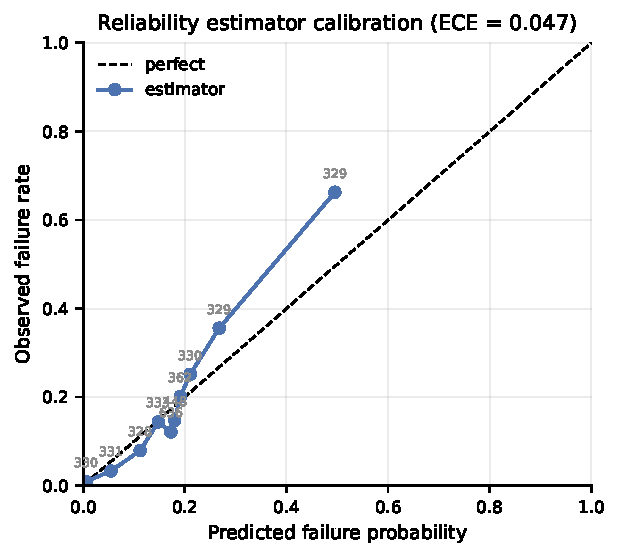
\includegraphics[width=0.8\textwidth]{fig_calibration}
\caption{Calibration of the failure-risk estimator, with expected calibration error.}
\label{fig:calibration}
\end{figure}

\subsection{What the corrections did}

Two rows carry the argument. \texttt{always\_correct} intervenes on every
instance and helps on \helpedAlwaysCorrect\% of them while harming
\harmedAlwaysCorrect\%, which is how a policy can be busy and still lose: the
harmful interventions are individually larger than the helpful ones. Our calibrated
gate intervenes on \rateRgc\% of instances and inverts that ratio, helping on
\helpedRgc\% of the instances it touches against \harmedRgc\% harmed, and its
oracle regret (\regretRgc{}) is the lowest of any acting policy.

That is the shape of the result throughout this paper. Restraint is what the gate
buys, not accuracy: it selects better than chance among the instances it acts on, and
still does not beat declining to act at all, because the actions available to it give
back more on the instances it gets wrong than they win on the instances it gets right.
Section~\ref{sec:decomposition} takes that apart.


Aggregate accuracy conceals the mechanism. Table~\ref{tab:decision} reports
decision-level quality, which only a counterfactual benchmark can produce: how often each
policy intervened, how often intervention helped rather than harmed, and the regret of
its choices against the oracle.

\begin{table}[htbp]
\centering
\caption{Decision quality. ``Helped'' and ``harmed'' are computed among corrected
instances only, so a policy can intervene frequently and still lose to never correcting.}
\label{tab:decision}
\small
\fittable{\begin{tabular}{lrrrrrrr}
\toprule
Policy & Corr. rate & Precision & Recall & F1 & Helped & Harmed & Regret \\
\midrule
never correct & 0.00 & --- & 0.000 & --- & --- & --- & 0.289 \\
rgc & 0.20 & 0.825 & 0.279 & 0.417 & 0.510 & 0.399 & 0.294 \\
random correct & 0.21 & 0.570 & 0.202 & 0.298 & 0.299 & 0.436 & 0.317 \\
threshold single & 0.29 & 0.606 & 0.296 & 0.398 & 0.188 & 0.268 & 0.350 \\
always correct & 1.00 & 0.592 & 1.000 & 0.744 & 0.264 & 0.292 & 0.378 \\
best fixed & 0.90 & 0.606 & 0.923 & 0.731 & 0.293 & 0.323 & 0.378 \\
\bottomrule
\end{tabular}
}
\end{table}

\begin{figure}[htbp]
\centering
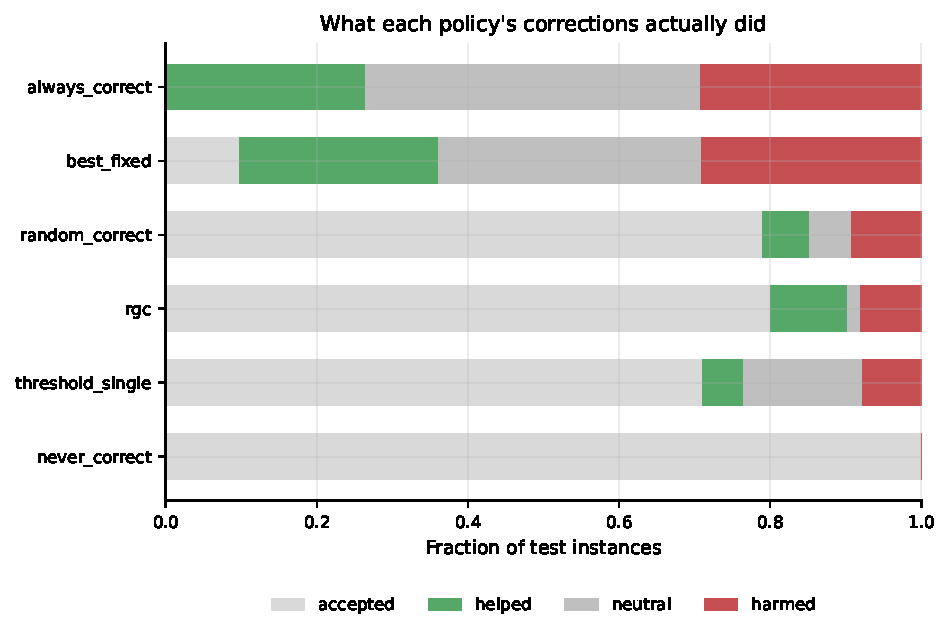
\includegraphics[width=0.8\textwidth]{fig_correction_outcomes}
\caption{Outcome of every intervention, by policy. What matters is not how often a policy
acts but how often acting was warranted.}
\label{fig:outcomes}
\end{figure}

\subsection{Three measurement pathologies}
\label{sec:pathologies}

Each of the following concealed the effect above, and we report them because any
evaluation of correction will encounter them.

\paragraph{Ratio gains explode.}
Expressing an action's value as $(\text{accept} - \text{action}) / \text{accept}$ divides
by an error that is sometimes near zero. On that scale the correlation between an
action's observed gain on one window and its realised gain on the next is $0.006$, with
residual standard deviations above $1000$: no usable signal. On the log scale
$\log(\text{accept}/\text{action})$, the identical data gives a correlation of $0.43$
with residual standard deviations below $0.7$, and a clear per-action structure. The
conclusion changes from ``correction is unpredictable'' to ``correction is predictable
for some actions and not others''.

\paragraph{The arithmetic mean describes the tail.}
MASE on this benchmark has a median near $0.6$ and a maximum near $190$; the worst 1\% of
instances carry roughly a fifth of the total error mass. Comparisons on the mean are
therefore comparisons of a few dozen instances. We report mean, offset geometric mean and
median throughout. Absolute geometric means depend on the additive offset used to handle
exact zeros; relative comparisons do not, and only relative comparisons are interpreted.

\paragraph{Oracle headroom is mostly selection bias.}
The unrestricted oracle, the minimum over all actions on each instance, advertises
large available improvement. But it selects the best of roughly ten noisy outcomes on a
single realisation, so much of that margin is the winner's curse. A \emph{realizable}
oracle, choosing the best action on validation origins and applying it to test, captures
almost none of it (Figure~\ref{fig:oracle}). Quoting the unrestricted figure would
overstate what any policy, including a perfect one, could attain.

\begin{figure}[htbp]
\centering
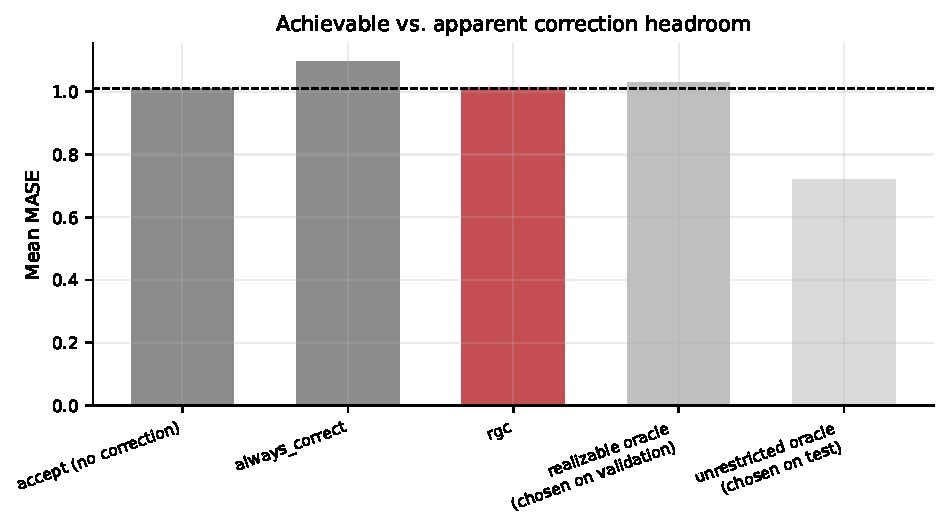
\includegraphics[width=0.8\textwidth]{fig_oracle_gap}
\caption{Accept, competing policies, and the two oracles. The unrestricted oracle is an
unattainable upper bound inflated by selection; the realizable oracle is attainable.}
\label{fig:oracle}
\end{figure}

\subsection{How much headroom is there? Most of the oracle gap is selection}
\label{sec:decomposition}

A common pattern in agentic forecasting systems is to diagnose a failure mode and apply
a repair matched to it \citep{tsscientist2025,nexus2026,castflow2026}. On synthetic
instances the generator's failure mode is known, so we can grant that pattern a perfect
diagnosis and ask what it is worth. Section~\ref{sec:headline} showed that the policies
we built do not beat a static ensemble; here we ask how much there was to gain at all.

\paragraph{Scope.}
This tests our ten-action space and our hand-designed mapping from failure mode to
candidate repairs (Section~\ref{sec:actionspace}). It is not a test of any published
system, none of which we re-implemented, and a richer action space or a learned mapping
could give a different answer.

\paragraph{Four stages, and two ways to select.}
We compare accepting the forecast; a \emph{canonical fix} that applies the first
repair our mapping assigns to the true failure mode; the best of that mode's two or
three matched candidates; and the best of all ten actions. The last two involve a
choice, and the choice can be made in two ways. Selecting on the \emph{test} outcomes
gives a ceiling that no policy could reach. Selecting on \emph{validation} origins and
scoring on held-out test origins, with the rule the realizable oracle uses (per series
and horizon, the action with the lowest mean validation error), gives what a policy
with perfect per-series knowledge could actually achieve. Table~\ref{tab:regretdecomp}
reports both, with series-level bootstrap intervals throughout.

\begin{table}[htbp]
\centering
\caption{The decomposition selected two ways, on \rdMaseNseries{} synthetic series with
ground-truth diagnosis. Rows 1--3 are percentage changes relative to accepting; rows 4--5
are differences between rows, in percentage points. Intervals are 95\% series-level
bootstrap; $\dagger$ marks one excluding zero. The canonical fix involves no
selection, so its two columns are identical. The left column minimises over test
outcomes, and the gap between the columns is the winner's curse.}
\label{tab:regretdecomp}
\small
\fittable{\begin{tabular}{llrr}
\toprule
Metric & Quantity & Selected on test (ceiling) & Selected on validation \\
\midrule
MASE & Canonical fix vs accept & 2.43~[-0.50, 5.33] & 2.43~[-0.50, 5.33] \\
MASE & Best of matched candidates vs accept & -15.12$^\dagger$~[-17.60, -12.80] & 5.33~[-3.20, 19.19] \\
MASE & Best of all actions vs accept (headroom) & -31.24$^\dagger$~[-33.46, -29.10] & 4.45$^\dagger$~[0.16, 9.95] \\
MASE & First-choice loss (pp) & 17.55$^\dagger$~[14.79, 20.50] & -2.90~[-16.62, 5.49] \\
MASE & Restriction loss (pp) & 16.12$^\dagger$~[14.49, 17.87] & 0.88~[-5.13, 9.89] \\
CRPS & Canonical fix vs accept & 3.59$^\dagger$~[0.03, 7.26] & 3.59$^\dagger$~[0.03, 7.26] \\
CRPS & Best of matched candidates vs accept & -19.52$^\dagger$~[-22.05, -17.01] & 3.76~[-6.54, 20.33] \\
CRPS & Best of all actions vs accept (headroom) & -33.42$^\dagger$~[-35.77, -31.11] & -0.80~[-4.24, 2.79] \\
CRPS & First-choice loss (pp) & 23.11$^\dagger$~[19.67, 26.83] & -0.17~[-16.69, 10.45] \\
CRPS & Restriction loss (pp) & 13.90$^\dagger$~[12.28, 15.70] & 4.56~[-4.44, 19.25] \\
\bottomrule
\end{tabular}
}
\end{table}

\paragraph{Selected on test, the headroom looks large; selected on validation, it is
gone.}
Minimising over test outcomes, the best action per instance improves MASE by
\rdMaseCeilTotalAbs\% over accepting, and the gap decomposes into two sizeable losses
(\rdMaseCeilFirst{} and \rdMaseCeilRestrict{} percentage points). That is the
decomposition an earlier version of this paper reported. It is an instance of the
selection-inflated oracle described in Section~\ref{sec:pathologies}: the expected
minimum of ten noisy outcomes is lower than the minimum of three, and the minimum of
three is lower than a single draw, even when no action carries any real signal.

Made on validation, the same choices recover nothing. The best action per series
changes MASE by \rdMaseRealTotal\% ([\rdMaseRealTotalCIlo, \rdMaseRealTotalCIhi]\%),
worse than accepting, and CRPS by \rdCrpsRealTotal\% ([\rdCrpsRealTotalCIlo,
\rdCrpsRealTotalCIhi]\%). Neither named loss is distinguishable from zero. Between
\rdCrpsCurseShare\% and \rdMaseCurseShare\% of the apparent headroom was selection.
Per-series repair choices do not transfer from earlier origins to later ones on this
benchmark, so there is no realizable headroom for a per-series policy to lose.

A pre-registered arm reaches the same answer independently. \texttt{best\_fixed},
fixed in the analysis plan before any result was seen, is exactly this realizable oracle
applied to all \nseries{} series, synthetic and real. It is significantly worse than
never correcting on MASE (\maseBestFixedVsNeverPct\%, [\maseBestFixedVsNeverCIlo,
\maseBestFixedVsNeverCIhi]\%). So the result does not rest on an analysis written after a
reviewer's objection; it was already in the pre-registered results, unremarked.

\paragraph{What survives.}
Three things, none of which depends on a test-selected quantity. First, under a perfect
diagnosis the canonical repair does not help: \rdMaseCanonical\% on MASE
([\rdMaseCanonicalCIlo, \rdMaseCanonicalCIhi]\%) and \rdCrpsCanonical\% on CRPS
([\rdCrpsCanonicalCIlo, \rdCrpsCanonicalCIhi]\%), the latter a significant
degradation. Second, choosing the best repair per series on validation does not help
either. Third, a single static ensemble applied everywhere does help on CRPS
(Section~\ref{sec:headline}), and it is the action validation selects when asked for
one static policy (Section~\ref{sec:staticcheck}). Choosing per series loses to
choosing once. That is the forecast-combination puzzle
\citep{stockwatson2004,smithwallis2009,claeskens2016} reappearing at the level of repair
selection: estimating which repair suits each series adds more variance than the
specificity recovers.

This also says something about how correction policies are usually evaluated. Oracle
regret against a test-selected oracle is the standard yardstick, and on this benchmark
almost all of what it measures is selection. A policy that closes half of such a gap
may have closed none of the realizable one.

% The LLM-arm results render only when scripts/llm_arms.py has actually produced
% them. Without that file the manuscript states plainly that the arms were not run,
% instead of rendering prose about results that do not exist. See ANALYSIS_PLAN.md D8.
\IfFileExists{tables/table_llm_arms.tex}{\subsection{Letting a language model decide}
\label{sec:llmarms}

Everything so far concerns policies whose decisions are made by arithmetic. But the
systems this paper is about delegate the decision to a language model, and a critique of
that architecture that never runs it would not be worth much. This section runs it.

Three arms share the counterfactual tensor with every policy above, so the outcome of
each action is identical and the only thing that varies is who chooses.
\texttt{llm\_single} sees the diagnostic evidence once and picks an action, the
Self-Refine pattern. \texttt{llm\_critique\_gate} sees the same evidence but first judges
\emph{whether} the forecast needs revising at all: the reflection step whose value is
this paper's question, and the mechanism \citet{huang2024selfcorrect} and
\citet{kamoi2024selfcorrect} found unreliable in reasoning tasks.
\texttt{rgc\_llm\_router} hands the model only the \emph{which}, keeping our quantitative
gate for the \emph{whether}, which separates the value of gating from the value of
routing. All three receive exactly the evidence our own gate receives: the comparison is
about how the decision is made, not about who saw more.

\paragraph{How this section relates to the previous one.}
Section~\ref{sec:decomposition} found no realizable per-series headroom: choosing
repairs on validation does not beat accepting. That sets the bar for a language model
in the decision loop. It cannot win by choosing repairs cleverly, because there is
little to win; it can only avoid losing by declining to act. The question this section
asks is therefore whether a model restrains itself, and the answer is that it does not.

\paragraph{Three model families, because one would not settle it.}
A single model failing to beat never-correcting invites the obvious reply that we picked
a weak one. The arms therefore run on unrelated families: \texttt{gemini-3.5-flash-lite},
a small hosted proprietary model, on one instance from each of the \nseries{} series;
\texttt{qwen3.8-27b}, an open-weight model of different lineage served by a different
provider, on 140 series; and \texttt{gpt-oss-20b}, an open-weight \emph{reasoning} model
run at medium effort, on \reasonSeries{} series. Free-tier quotas set the coverage and they meter differently ---
one provider caps requests per day, the other tokens per day --- so the series count is
given per row in Table~\ref{tab:llmarms}, and the smaller family covers the two arms that
carry the argument rather than all three. Every non-LLM arm is re-scored within its own
family's subsample, so rows are comparable down a block but not across blocks.
Temperature is 0 throughout and every response is cached, so the experiment replays
without an API key.

The first two are not reasoning models and receive no prompt engineering: the evidence
block is a fixed template and each decision is a single zero-shot turn. The third
deliberates explicitly, and a fourth condition described below shows a model worked
examples drawn from the validation split. What the families establish together is
therefore not a claim about language models in general, but that the result is not an
artefact of one model's idiosyncrasies, of an absence of deliberation, or of the
zero-shot setting, which are the three objections a single-family null cannot answer.

\begin{table}[htbp]
\centering
\caption{LLM correction arms against the same counterfactual outcomes, for two model
families. Non-LLM arms are re-scored within each family's own subsample, so rows are
comparable within a family block but not across blocks; the covered series count is given
per row. Effects are series-level differences from never correcting with 95\% bootstrap
intervals; $\dagger$ marks an interval excluding zero. Negative favours the policy.
``LLM calls'' is the live provider call count, since a correction stage that does not
help is still not free.}
\label{tab:llmarms}
\small
\fittable{\begin{tabular}{lllrrrrrr}
\toprule
Metric & Model & Policy & Series & Series mean & $\Delta$ & 95\% CI & Win rate & LLM calls \\
\midrule
Point (MASE) & Gemini 3.5 Flash-Lite & never correct & 578 & 1.2220 & 0.00\% & [0.00, 0.00] & 50.0\% & 0 \\
Point (MASE) & Gemini 3.5 Flash-Lite & always ensemble & 578 & 1.1520 & -5.73\%$^\dagger$ & [-9.54, -1.99] & 53.9\% & 0 \\
Point (MASE) & Gemini 3.5 Flash-Lite & rgc calibrated & 578 & 1.2196 & -0.19\% & [-0.72, 0.26] & 50.3\% & 0 \\
Point (MASE) & Gemini 3.5 Flash-Lite & llm single & 578 & 1.3243 & 8.37\%$^\dagger$ & [3.29, 13.94] & 42.2\% & 0 \\
Point (MASE) & Gemini 3.5 Flash-Lite & llm critique gate & 578 & 1.3136 & 7.50\%$^\dagger$ & [2.73, 12.89] & 42.8\% & 288 \\
Point (MASE) & Gemini 3.5 Flash-Lite & rgc llm router & 578 & 1.2814 & 4.87\%$^\dagger$ & [0.95, 10.06] & 47.5\% & 258 \\
Point (MASE) & Gemini 3.5 Flash-Lite & always correct & 578 & 1.2920 & 5.73\% & [-0.48, 14.43] & 47.1\% & 0 \\
Probabilistic (CRPS) & Gemini 3.5 Flash-Lite & never correct & 578 & 1.0629 & 0.00\% & [0.00, 0.00] & 50.0\% & 0 \\
Probabilistic (CRPS) & Gemini 3.5 Flash-Lite & always ensemble & 578 & 0.9503 & -10.59\%$^\dagger$ & [-15.14, -6.70] & 53.8\% & 0 \\
Probabilistic (CRPS) & Gemini 3.5 Flash-Lite & rgc calibrated & 578 & 1.0064 & -5.31\%$^\dagger$ & [-9.36, -1.91] & 53.5\% & 0 \\
Probabilistic (CRPS) & Gemini 3.5 Flash-Lite & llm single & 578 & 1.1530 & 8.48\%$^\dagger$ & [3.00, 14.55] & 43.9\% & 0 \\
Probabilistic (CRPS) & Gemini 3.5 Flash-Lite & llm critique gate & 578 & 1.1493 & 8.13\%$^\dagger$ & [3.17, 13.92] & 44.3\% & 288 \\
Probabilistic (CRPS) & Gemini 3.5 Flash-Lite & rgc llm router & 578 & 1.1015 & 3.63\%$^\dagger$ & [0.48, 8.04] & 48.7\% & 258 \\
Probabilistic (CRPS) & Gemini 3.5 Flash-Lite & always correct & 578 & 1.0979 & 3.29\% & [-4.92, 13.64] & 51.6\% & 0 \\
Point (MASE) & Qwen3.8-27B (Groq) & never correct & 140 & 0.8936 & 0.00\% & [0.00, 0.00] & 50.0\% & 0 \\
Point (MASE) & Qwen3.8-27B (Groq) & always ensemble & 140 & 0.8892 & -0.50\% & [-5.17, 4.69] & 51.4\% & 0 \\
Point (MASE) & Qwen3.8-27B (Groq) & rgc calibrated & 140 & 0.8850 & -0.96\% & [-2.85, 0.00] & 50.7\% & 0 \\
Point (MASE) & Qwen3.8-27B (Groq) & llm single & 140 & 0.9400 & 5.19\%$^\dagger$ & [0.86, 10.19] & 46.8\% & 0 \\
Point (MASE) & Qwen3.8-27B (Groq) & llm critique gate & 140 & 0.9458 & 5.85\%$^\dagger$ & [1.45, 10.84] & 45.7\% & 11 \\
Probabilistic (CRPS) & Qwen3.8-27B (Groq) & never correct & 140 & 0.7513 & 0.00\% & [0.00, 0.00] & 50.0\% & 0 \\
Probabilistic (CRPS) & Qwen3.8-27B (Groq) & always ensemble & 140 & 0.7168 & -4.59\% & [-10.64, 0.96] & 52.1\% & 0 \\
Probabilistic (CRPS) & Qwen3.8-27B (Groq) & rgc calibrated & 140 & 0.7097 & -5.54\%$^\dagger$ & [-10.73, -0.69] & 57.1\% & 0 \\
Probabilistic (CRPS) & Qwen3.8-27B (Groq) & llm single & 140 & 0.7941 & 5.70\% & [-0.48, 12.33] & 48.6\% & 0 \\
Probabilistic (CRPS) & Qwen3.8-27B (Groq) & llm critique gate & 140 & 0.7892 & 5.04\% & [-1.22, 11.81] & 50.7\% & 11 \\
Point (MASE) & GPT-OSS-20B reasoning (Groq) & never correct & 60 & 1.0447 & 0.00\% & [0.00, 0.00] & 50.0\% & 0 \\
Point (MASE) & GPT-OSS-20B reasoning (Groq) & always ensemble & 60 & 1.0974 & 5.04\% & [-9.06, 24.71] & 48.3\% & 0 \\
Point (MASE) & GPT-OSS-20B reasoning (Groq) & rgc calibrated & 60 & 1.0454 & 0.06\% & [-0.16, 0.34] & 50.0\% & 0 \\
Point (MASE) & GPT-OSS-20B reasoning (Groq) & llm single & 60 & 1.1024 & 5.52\% & [-2.92, 14.61] & 50.0\% & 60 \\
Point (MASE) & GPT-OSS-20B reasoning (Groq) & llm critique gate & 60 & 1.1034 & 5.62\% & [-3.77, 15.32] & 47.5\% & 60 \\
Probabilistic (CRPS) & GPT-OSS-20B reasoning (Groq) & never correct & 60 & 0.9179 & 0.00\% & [0.00, 0.00] & 50.0\% & 0 \\
Probabilistic (CRPS) & GPT-OSS-20B reasoning (Groq) & always ensemble & 60 & 0.8967 & -2.31\% & [-16.91, 13.54] & 53.3\% & 0 \\
Probabilistic (CRPS) & GPT-OSS-20B reasoning (Groq) & rgc calibrated & 60 & 0.9341 & 1.76\% & [-3.18, 7.54] & 51.7\% & 0 \\
Probabilistic (CRPS) & GPT-OSS-20B reasoning (Groq) & llm single & 60 & 0.9776 & 6.49\% & [-2.30, 15.67] & 42.5\% & 60 \\
Probabilistic (CRPS) & GPT-OSS-20B reasoning (Groq) & llm critique gate & 60 & 0.9805 & 6.81\% & [-1.72, 15.52] & 43.3\% & 60 \\
Point (MASE) & Gemini 3.5 Flash-Lite, 8-shot & never correct & 60 & 1.0447 & 0.00\% & [0.00, 0.00] & 50.0\% & 0 \\
Point (MASE) & Gemini 3.5 Flash-Lite, 8-shot & always ensemble & 60 & 1.0974 & 5.04\% & [-9.06, 24.71] & 48.3\% & 0 \\
Point (MASE) & Gemini 3.5 Flash-Lite, 8-shot & rgc calibrated & 60 & 1.0454 & 0.06\% & [-0.16, 0.34] & 50.0\% & 0 \\
Point (MASE) & Gemini 3.5 Flash-Lite, 8-shot & llm single & 60 & 1.1142 & 6.65\% & [-1.25, 15.77] & 45.8\% & 0 \\
Point (MASE) & Gemini 3.5 Flash-Lite, 8-shot & llm critique gate & 60 & 1.3462 & 28.85\% & [-0.49, 80.30] & 46.7\% & 0 \\
Probabilistic (CRPS) & Gemini 3.5 Flash-Lite, 8-shot & never correct & 60 & 0.9179 & 0.00\% & [0.00, 0.00] & 50.0\% & 0 \\
Probabilistic (CRPS) & Gemini 3.5 Flash-Lite, 8-shot & always ensemble & 60 & 0.8967 & -2.31\% & [-16.91, 13.54] & 53.3\% & 0 \\
Probabilistic (CRPS) & Gemini 3.5 Flash-Lite, 8-shot & rgc calibrated & 60 & 0.9341 & 1.76\% & [-3.18, 7.54] & 51.7\% & 0 \\
Probabilistic (CRPS) & Gemini 3.5 Flash-Lite, 8-shot & llm single & 60 & 0.9944 & 8.33\%$^\dagger$ & [0.49, 16.66] & 40.0\% & 0 \\
Probabilistic (CRPS) & Gemini 3.5 Flash-Lite, 8-shot & llm critique gate & 60 & 1.1299 & 23.09\%$^\dagger$ & [1.96, 58.52] & 39.2\% & 0 \\
Point (MASE) & Gemini 3.5 Flash-Lite, 0-shot (matched) & never correct & 60 & 1.0447 & 0.00\% & [0.00, 0.00] & 50.0\% & 0 \\
Point (MASE) & Gemini 3.5 Flash-Lite, 0-shot (matched) & always ensemble & 60 & 1.0974 & 5.04\% & [-9.06, 24.71] & 48.3\% & 0 \\
Point (MASE) & Gemini 3.5 Flash-Lite, 0-shot (matched) & rgc calibrated & 60 & 1.0454 & 0.06\% & [-0.16, 0.34] & 50.0\% & 0 \\
Point (MASE) & Gemini 3.5 Flash-Lite, 0-shot (matched) & llm single & 60 & 1.1330 & 8.45\%$^\dagger$ & [3.00, 14.72] & 39.2\% & 50 \\
Point (MASE) & Gemini 3.5 Flash-Lite, 0-shot (matched) & llm critique gate & 60 & 1.1407 & 9.19\%$^\dagger$ & [1.69, 17.60] & 38.3\% & 50 \\
Probabilistic (CRPS) & Gemini 3.5 Flash-Lite, 0-shot (matched) & never correct & 60 & 0.9179 & 0.00\% & [0.00, 0.00] & 50.0\% & 0 \\
Probabilistic (CRPS) & Gemini 3.5 Flash-Lite, 0-shot (matched) & always ensemble & 60 & 0.8967 & -2.31\% & [-16.91, 13.54] & 53.3\% & 0 \\
Probabilistic (CRPS) & Gemini 3.5 Flash-Lite, 0-shot (matched) & rgc calibrated & 60 & 0.9341 & 1.76\% & [-3.18, 7.54] & 51.7\% & 0 \\
Probabilistic (CRPS) & Gemini 3.5 Flash-Lite, 0-shot (matched) & llm single & 60 & 0.9981 & 8.73\%$^\dagger$ & [2.75, 15.62] & 38.3\% & 50 \\
Probabilistic (CRPS) & Gemini 3.5 Flash-Lite, 0-shot (matched) & llm critique gate & 60 & 1.0195 & 11.06\%$^\dagger$ & [4.34, 18.85] & 34.2\% & 50 \\
\bottomrule
\end{tabular}
}
\end{table}

\paragraph{On the primary family, every LLM arm is worse than doing nothing.}
On the primary family all
three arms degrade both metrics with intervals that exclude zero: a single pass costs
\llmMaseLlmSinglePct\% MASE ([\llmMaseLlmSingleCIlo, \llmMaseLlmSingleCIhi]\%) and
\llmCrpsLlmSinglePct\% CRPS ([\llmCrpsLlmSingleCIlo, \llmCrpsLlmSingleCIhi]\%); the
self-critique gate costs \llmMaseLlmCritiqueGatePct\% and
\llmCrpsLlmCritiqueGatePct\%, and even the router, which acts on only a seventh of
instances because our quantitative gate holds it back, costs
\llmMaseRgcLlmRouterPct\% and \llmCrpsRgcLlmRouterPct\%. Each wins on fewer than half of
series. On the same instances the static ensemble improves CRPS by
\llmCrpsAlwaysEnsembleAbs\% ([\llmCrpsAlwaysEnsembleAbsCIlo,
\llmCrpsAlwaysEnsembleAbsCIhi]\%), so the subsample is not too small to resolve a real
effect; it resolves one, in the opposite direction from the arms that reason about each
instance.

\paragraph{A discrepancy between two designs.}
In Table~\ref{tab:llmarms} the static ensemble's MASE advantage clears significance,
whereas in Table~\ref{tab:headline} the same policy's MASE interval includes zero. The
tables are computed on different data: the headline analysis uses every test origin
(\ntestinstances{} instances), while these arms use one randomly chosen origin per series,
because that is what the API budget allowed. Both are series-level and both are correct
for what they cover; the subsample simply draws fewer of the extreme origins that widen
the full interval. \textbf{The headline analysis is the primary one}, and the claim we
stand behind is the more conservative of the two: that no policy reliably improves
point accuracy. We flag the difference because quoting the subsample's narrower interval
as though it settled the point would be exactly the kind of selection this paper
criticises elsewhere.

The decision-level view explains the aggregate. When the language model chooses to
correct, it makes the forecast \emph{worse} on roughly half the instances it touches and
better on under a third: it harms about $1.8\times$ as often as it helps. The router
is the worst offender at a $64\%$ harm rate, which is initially surprising until one
notices what it means: even after a calibrated gate has correctly identified an instance
worth correcting, delegating the choice of \emph{which} repair to a language model
destroys the opportunity. That is Section~\ref{sec:decomposition}'s restriction-and-first-choice
loss appearing again, with a language model in the role of the fixed canonical mapping.
A better-informed guess is still a guess; it is not a measurement.

\paragraph{The reflection step carries almost no information.}
We expected the comparison between \texttt{llm\_single} and \texttt{llm\_critique\_gate}
to be the sharpest in this section, because they differ in exactly one thing: whether the
model is asked to judge the need for correction before choosing. It is not sharp at all.
Asked plainly whether the forecast needs revising, the model answers yes on
\rateLlmCritiqueGate\% of instances, almost exactly the rate at which the single-pass arm
chooses to act anyway, and the two arms land within a percentage point of each other on
both metrics.

Matching rates would be weak evidence on its own; two arms can intervene equally often
while selecting very different instances, one of them well. So we test discrimination
directly, against the benchmark's ground-truth \texttt{should\_correct} label
(Table~\ref{tab:discrimination}). The critique's yes/no separates warranted from
unwarranted correction at AUROC \discrimAurocCritique{}, against a chance value of 0.500.
Its selection precision is \discrimPrecisionCritique\%, where the base rate is
\discrimBaseRate\% and a coin firing at the same rate achieves \discrimPrecisionRandom\%.
And \discrimJaccard\% of the instances it elects to correct are the same instances the
uncritiqued arm corrects.

The decisive comparison is with the arm that does no critique at all, which discriminates
at AUROC \discrimAurocSingle{}. \textbf{Adding an explicit reflection step moves
discrimination by \discrimAurocDelta{}; from near-chance to near-chance.} The critique
is not merely a weak gate; it is very nearly a re-description of what the model would have
done without being asked. Both families show the same pattern
(Table~\ref{tab:discrimination}), including one where the critique step \emph{raises} the
intervention rate instead of leaving it flat, and still adds essentially nothing to
discrimination.

\paragraph{The same judgement, made arithmetically.}
The natural question is whether this decision is simply hard. It is not. Our reliability
estimator --- gradient boosting over the same diagnostic features the model was shown in
prose, fitted on validation only --- scores \discrimAurocArithmetic{} against the
\emph{same} label on the \emph{same} instances (Table~\ref{tab:discrimination}). That is
\discrimArithmeticAdvantage{} AUROC above the self-critique. We deliberately do not
express that as a multiple of the critique's distance from chance: dividing by a
near-zero baseline is the first of the measurement pathologies this paper documents
(Section~\ref{sec:pathologies}). We also
report the contrast \emph{matched}, because the triage figure quoted in
Section~\ref{sec:triage} targets a different label, and setting the two against each
other directly would not be legitimate.

\paragraph{What that contrast does and does not license.}
A binary yes/no scored as an AUROC is balanced accuracy, and nothing more. The
estimator emits a continuous score, so scoring the two the same way credits it for
ranking that a yes/no cannot express, and some of the apparent gap is an artefact of
the output type rather than of the judgement behind it. The contrast is therefore reported at matched footing in two ways, both in
Table~\ref{tab:discrimination}.

The first gives the language model the same kind of credit. Its verbalised confidence
is continuous, so it can be scored as a ranking against the same label: it reaches
AUROC \discrimAurocLlmConfidence{} against the estimator's \discrimAurocArithmetic{},
a gap of \discrimContinuousGap{}. The second removes the ranking question entirely
by forcing both to the same operating point --- the estimator thresholded to flag
exactly the fraction of instances the critique gate flags --- and compares balanced
accuracy: \discrimBalaccArithmetic{} against \discrimBalaccCritique{}, a gap of
\discrimMatchedGap{}.

The two ask different questions and both are worth keeping. (a) asks whether the
model's stated risk can \emph{rank} instances at all, independent of where a threshold
would be placed. (b) asks how much better the decision is at the rate the model
actually fires, which is the quantity a deployed gate delivers. It is worth noting that
(a) is marginally \emph{larger} than the unmatched comparison it replaces
(\discrimContinuousGap{} against \discrimArithmeticAdvantage{}), so matching was not a
route to a smaller number; only (b), which removes the ranking question entirely,
narrows the gap.

At a matched operating point the gap
is \discrimMatchedGap{}, not the \discrimArithmeticAdvantage{} a naive reading of the
first two columns would give. The artefact was real and it was worth roughly a third
of the apparent difference. What survives it is still the finding: on the same
instances, against the same label, at the same rate of intervention, a gradient-boosted
model over a few dozen scalar diagnostics decides substantially better than a language
model reasoning over the same evidence in words.

What the contrast does not license is a claim that language models cannot do this. The
estimator is fitted on the validation split and the model is not, and that asymmetry is
addressed directly below. Nor does it license a claim about relative ceilings: it
compares one fitted estimator against one prompted model, at one budget, and a
different prompt or a different model could land elsewhere. It licenses exactly one
thing, which is the thing the deployment question turns on: that the cheap
arithmetic option available to any practitioner today is the better of the two.


\begin{table}[htbp]
\centering
\caption{Does verbal self-critique carry information about whether to correct? All
columns are computed on the same instances against the same ground-truth
\texttt{should\_correct} label. ``AUROC (critique)'' scores a binary yes/no and is
therefore balanced accuracy; ``AUROC (arithmetic)'' scores a continuous estimator and
is credited for ranking, so the two are compared at matched footing in the text rather
than by subtracting these columns. $\Delta$ AUROC is the within-model quantity the
claim rests on: the same model, the same instances, deciding with and without being
asked to reflect. ``Overlap'' is the Jaccard overlap of the two intervention sets.}
\label{tab:discrimination}
\small
\fittable{\begin{tabular}{lrrrrrrrrr}
\toprule
Model & $n$ & Base rate & AUROC (critique) & AUROC (no critique) & $\Delta$ AUROC & AUROC (arithmetic) & Precision & Random & Overlap \\
\midrule
Gemini 3.5 Flash-Lite & 578 & 59.7\% & 0.532 & 0.522 & 0.010 & 0.760 & 61.9\% & 59.9\% & 82\% \\
Qwen3.8-27B (Groq) & 140 & 52.9\% & 0.568 & 0.561 & 0.008 & 0.693 & 59.0\% & 51.4\% & 75\% \\
GPT-OSS-20B reasoning (Groq) & 60 & 60.0\% & 0.493 & 0.590 & -0.097 & 0.774 & 59.6\% & 60.0\% & 80\% \\
\bottomrule
\end{tabular}
}
\end{table}

\paragraph{Why it intervenes so often: it thinks its forecasts are far worse than
they are.}
The arms are asked, in the same breath as the decision, for a number between 0 and 1
expressing how reliable they judge the current forecast to be. That is a claim about
exactly the event the reliability estimator predicts, so the two can be scored against
each other on identical instances and an identical label. This is pre-registered
hypothesis H5, and it is \textbf{supported}: the estimator's calibration error is
\calEceDiff{} lower ([\calEceDiffCIlo, \calEceDiffCIhi], bootstrapped over series),
and the same ordering holds on the Brier score.

The size and direction of the miscalibration are what matter here. Large errors occur
on \calBaseRate\% (on the \calN-instance subsample the LLM arms run on) of these instances; the model's stated risk averages
\calLlmMeanRisk{}. It believes its forecasts fail roughly two and a half times as often
as they do. That is not a detail about calibration, it is the mechanism behind the
headline: a model that thinks most of its forecasts are unreliable will conclude that
most of them need fixing, which is precisely the disposition the intervention rates
show. The reflection step is not failing to detect a problem it should have seen: it is reporting a problem that is mostly not there.

Table~\ref{tab:calibration} also contains the reason we do not rest this on calibration
error alone. A constant predictor that simply emits the base rate attains an ECE of
essentially zero while ranking nothing at all, and its Brier score (\calConstBrier{})
is nonetheless better than the language model's (\calLlmBrier{}). By the proper
scoring rule, the agent's stated confidence is worse than a constant. It is not
worthless as a \emph{ranking}: its AURC of \calLlmAurc{} beats the constant's
\calConstAurc{}, so there is some signal in which forecasts it doubts most. But that
signal is buried under a bias large enough to make the resulting decisions wrong, and a
gate reads the level, not the ranking.

That a language model's stated confidence is poorly calibrated is not itself news
\citep{kadavath2022know,lin2022verbalized,xiong2024confidence}, and we do not present it
as such. Two things here are worth separating from that literature. The direction is
inverted: the usual finding is overconfidence, a model claiming more certainty than its
accuracy warrants, whereas this model is systematically \emph{pessimistic} about the
artefact it is judging. And the consequence is operational rather than presentational.
In the settings where verbalised confidence is normally studied it is a number shown to
a reader, who may discount it; here it is wired into a control loop, where a bias of
this size does not mislead anyone so much as it manufactures roughly one unnecessary
repair for every instance that needed one.

\begin{table}[htbp]
\centering
\caption{H5: the agent's stated confidence against a calibrated estimate of the same
event. Both predict the probability of a large error, on the same \calN{} instances
and against the same label; lower is better in every column. The constant predictor is
included deliberately: it attains a perfect calibration error while ranking nothing,
which is why ECE is never read here on its own.}
\label{tab:calibration}
\small
\fittable{\begin{tabular}{lrrrr}
\toprule
Predictor & ECE & Brier & AURC & Mean $p$ \\
\midrule
LLM verbalised confidence & 0.3254 & 0.3148 & 0.1593 & 0.544 \\
Reliability estimator (calibrated) & 0.0502 & 0.1401 & 0.0883 & 0.185 \\
Constant at base rate (0.22) & 0.0000 & 0.1714 & 0.2291 & 0.220 \\
\bottomrule
\end{tabular}
}
\end{table}

\paragraph{Deliberation, and demonstration, against criteria fixed in advance.}
Two reasonable objections are still open at this point. The models run so far answer in a
single zero-shot turn, so the failure could be an absence of deliberation instead of a
property of the mechanism. And the arithmetic comparator is fitted on the validation
split while the language model is shown nothing, so the contrast above could be measuring
supervision rather than capability. Both were tested on one shared denominator ---
\reasonSeries{} series, one origin each --- with the falsification criteria written down
before the runs completed (deviation~D9). The deliberation arm is \texttt{gpt-oss-20b} at
\texttt{reasoning\_effort} \texttt{= medium}, with a completion budget large enough for
the reasoning trace and the answer; it recorded no provider failures and no unparsed
replies. The demonstration arm prepends eight worked examples drawn from validation and
labelled by the counterfactual tensor --- the same supervision, out of the same data, that
the estimator receives --- and runs against a matched zero-shot control on the identical
series, so the comparison is within-model on the same instances.

Neither closes the gap. The reasoning model degrades MASE by \reasonMaseSinglePct\%
([\reasonMaseSingleCIlo, \reasonMaseSingleCIhi]\%) in one pass and
\reasonMaseCritiquePct\% ([\reasonMaseCritiqueCIlo, \reasonMaseCritiqueCIhi]\%) with
self-critique, intervening on \reasonRateSingle\% and \reasonRateCritique\% of instances
respectively: the highest rates of any family. Eight worked examples move the
intervention rate from \zeroshotRateSingle\% to \fewshotRateSingle\% and the effect on
MASE from \zeroshotMaseSinglePct\% ([\zeroshotMaseSingleCIlo,
\zeroshotMaseSingleCIhi]\%, excluding zero) to \fewshotMaseSinglePct\%
([\fewshotMaseSingleCIlo, \fewshotMaseSingleCIhi]\%, no longer excluding zero). That is a small improvement this denominator cannot resolve, not a repair: the
two intervals overlap over almost their whole length, and the demonstration condition does
not bring the arm to parity with never correcting. The critique gate is a different story, and it runs against us. With the same eight
examples its degradation grew rather than shrank: from \zeroshotMaseCritiquePct\% to
\fewshotMaseCritiquePct\% on MASE ([\fewshotMaseCritiqueCIlo, \fewshotMaseCritiqueCIhi]\%)
and from \zeroshotCrpsCritiquePct\% to \fewshotCrpsCritiquePct\% on CRPS
([\fewshotCrpsCritiqueCIlo, \fewshotCrpsCritiqueCIhi]\%, excluding zero). The MASE
interval is wide enough that a few series drive it, but the direction is unambiguous:
showing the gate worked examples made it more harmful, not less. We do not have an
explanation we can test. What it does rule out is the reading that the critique gate
failed only for want of supervision.

The obvious question is why the demonstration condition stopped at eight examples and
\fewshotSeries{} series. The answer is budget rather than design: the prefix multiplies
prompt tokens roughly sixfold, and free-tier quotas bind on tokens for one provider and
on requests for the other. A larger demonstration budget, or in-context examples
selected per instance rather than fixed, is untested here and is the version of this
arm we would run first with more compute. What we can say is that the cheapest form of
the intervention, the one a practitioner would reach for, does not restrain the
model, and that is a narrower claim than the arm was built to make.

The pre-registered falsifiers did not fire. The primary one asked whether self-critique
would raise this model's discrimination by more than $+0.05$ AUROC over the same model
deciding without reflection. It moved by \reasonAurocDelta{}: \emph{down}, from
\reasonAurocSingle{} to \reasonAurocCritique{}, on \reasonDiscrimN{} instances where the
arithmetic estimator scored \reasonAurocArithmetic{} against the identical label. This is
the strongest form of the within-model result in the paper. Asking the one model that
actually deliberates to deliberate about its own judgement did not improve that judgement;
it made it slightly worse.

\paragraph{Given the decision to correct, is the chosen repair any good?}
The arms conflate two decisions: whether to correct, and which repair to apply. The
tensor separates them, because it holds the outcome of every action on every instance.
On the instances where an arm intervened we compare the repair it chose against a
uniform draw from the same menu on the same instance, computed exactly by averaging the
menu's outcomes. That comparison involves no selection, so it is the one the claims rest
on (Table~\ref{tab:actionchoice}).

On the primary family the choice cannot be told apart from the coin. Single-pass
selection scores \actionChoiceSinglePct\% relative to a uniform draw
([\actionChoiceSingleCIlo, \actionChoiceSingleCIhi]\%) and the critique arm
\actionChoiceCritiquePct\% ([\actionChoiceCritiqueCIlo, \actionChoiceCritiqueCIhi]\%).
Having decided to act, the model's choice of repair carries no measurable advantage over
choosing at random among the options it was shown.

The table also shows the best action in each menu. That row is a maximum over test
outcomes, and Section~\ref{sec:decomposition} shows such maxima are almost entirely
winner's curse on this benchmark, so it is context rather than a target, and no claim
uses it. The router arm's \actionChoiceRouterPct\% rests on \actionChoiceRouterN{}
instances with an interval of [\actionChoiceRouterCIlo, \actionChoiceRouterCIhi]\%; it
is underpowered and excluded from claims.

\begin{table}[htbp]
\centering
\caption{Given the decision to correct, how good is the chosen repair? MASE on the
instances where each arm intervened. The uniform draw averages the menu's outcomes
exactly and is the comparison claims rest on. The best-in-menu row is a maximum over
test outcomes, inflated by selection (Section~\ref{sec:decomposition}), and is shown
for context only. Intervals are series-level bootstrap; the router arm is underpowered.}
\label{tab:actionchoice}
\small
\fittable{\begin{tabular}{lrrr}
\toprule
 & LLM single & LLM critique gate & RGC + LLM router \\
\midrule
Instances intervened on & 361 & 367 & 80 \\
Best in menu (test-selected ceiling) & 0.6487 & 0.6273 & 0.5067 \\
\textbf{Model's chosen action} & \textbf{1.1190} & \textbf{1.0906} & \textbf{1.4109} \\
Uniform draw from same menu & 1.0806 & 1.0678 & 1.0996 \\
Worst action in menu & 2.0608 & 2.0461 & 2.5194 \\
\midrule Chosen vs.\ uniform draw & 3.55\%~[-4.07, 12.11] & 2.13\%~[-5.17, 10.66] & 28.31\%~[-0.99, 65.84] \\
\bottomrule
\end{tabular}
}
\end{table}

\paragraph{The reasoning model may choose better, but it still acts too often.}
The reasoning family points the other way on this test. Its single-pass choice scores
\reasonChoiceSinglePct\% against a uniform draw ([\reasonChoiceSingleCIlo,
\reasonChoiceSingleCIhi]\%) and its critique arm \reasonChoiceCritiquePct\%
([\reasonChoiceCritiqueCIlo, \reasonChoiceCritiqueCIhi]\%). Both intervals just
include zero at \reasonSeries{} series, so this is a direction, not an effect. If it
holds, deliberation helps with which repair to apply and not with whether to apply one;
and because this arm still intervenes on \reasonRateSingle\% of instances, its net
effect on accuracy stays negative either way.

\paragraph{The pre-registered test of H7.}
H7 asked whether a quantitative gate decides better than verbal self-critique, scored by
oracle regret. It is the one hypothesis in the plan that could not be evaluated until
these arms ran. It is \textbf{\verdictHSeven}: the calibrated gate's mean regret is
\statHSeven{} lower than the LLM critique gate's. The comparison is worth stating
carefully, because the gate achieves this largely by declining to act; its regret is
almost identical to never correcting. The finding is therefore not that quantitative
gating is good at choosing corrections. It is that it is good at \emph{not} choosing
them, and that verbal self-critique is not.

\paragraph{What this does not establish.}
Three families, a reasoning model at real effort, and a demonstration condition close the
cheapest objections but not every one. We cannot rule out that a frontier reasoning model,
multi-turn deliberation with tool access during the decision, or a prompt engineered
against this benchmark would do better; nor that a larger member of the same reasoning
family --- the one originally planned, lost to a daily token cap --- would separate from
the 20B model we ran. The reasoning and demonstration conditions cover \reasonSeries{}
series, which is enough to replicate a direction and not enough to establish an effect on
its own. Nor did we test sensitivity to prompt wording, and the pessimism result in particular
may depend on how the confidence question is phrased. What the result does establish
is narrower: the mechanism
\emph{as commonly deployed}, on the evidence commonly available to it, is not merely
unhelpful but reliably harmful; its harm resolves at the primary family's sample size, while the two smaller families show the same direction without resolving it. Self-reflection, the intervention most often proposed as the fix, did not improve the model's judgement in any family we ran.

\paragraph{The cost side.}
These are also the expensive arms. The self-critique gate alone made
\llmCallsCritiqueGate{} live provider calls, and the three arms together consumed
\llmCallsTotal{} calls and \llmPromptTokensThousands{}k prompt tokens on the primary
family. The static ensemble that outperforms all of them makes zero
provider calls and takes no per-instance decision whatsoever. Any argument for an
LLM-in-the-loop correction stage has to be made against that baseline, and on this
benchmark it cannot be made on accuracy at any price.
}{%
\subsection{Letting a language model decide}
\label{sec:llmarms}

\emph{This section is intentionally empty in the present build.} The arms that delegate
the correction decision to a language model --- a single-pass chooser, a verbal
self-critique gate, and a gate-plus-LLM-router --- are implemented, tested end to end,
and run with one command against the same counterfactual tensor as every policy above.
They are not reported here because the provider's free tier allows 500 requests per day
for the configured model and 20 for the alternative, and a run covering enough series to
support a series-level interval needs several times that. Deviation~D8 in the analysis
plan records the constraint and what was cached.

We flag this prominently instead of burying it: this manuscript argues about
architectures that delegate correction to a language model, and until these arms are
reported that argument rests on the decomposition in
Section~\ref{sec:decomposition} and on the non-LLM policies, not on direct evidence about
language-model decision-making. A reader should discount the paper's claims about verbal
self-critique accordingly.
}

\subsection{Selective prediction: a positive, deployable finding}
\label{sec:triage}

The results above are cautionary about automated correction. The failure-risk estimator
that drives the gate is nonetheless independently useful for a different and arguably
more common industrial purpose: prioritising forecasts for human review. Because the
estimator is fit and evaluated exactly as in Section~\ref{sec:decomposition} (validation
only, never test), the numbers below describe a deployable capability instead of a
ceiling.

\begin{table}[htbp]
\centering
\caption{Selective-prediction value of the failure-risk estimator (AUROC
$=\triageauroc$, base rate of large errors $=\triagebaserate\%$). Reviewing the
riskiest 10\% of forecasts catches roughly a third of all large errors at two-thirds
precision -- a $\triageliftPOneZero\times$ enrichment over reviewing at random.}
\label{tab:triage}
\small
\fittable{\begin{tabular}{lrrrr}
\toprule
Review budget & Reviewed & Precision & Recall & Lift \\
\midrule
5.0\% & 164 & 0.762 & 0.190 & 3.81$\times$ \\
10.0\% & 328 & 0.665 & 0.332 & 3.32$\times$ \\
20.0\% & 656 & 0.511 & 0.510 & 2.55$\times$ \\
30.0\% & 985 & 0.424 & 0.636 & 2.12$\times$ \\
50.0\% & 1642 & 0.322 & 0.805 & 1.61$\times$ \\
\bottomrule
\end{tabular}
}
\end{table}

This reframes what the benchmark's reliability estimation contributes: not necessarily
\emph{automated} self-correction, which our results treat with substantial scepticism,
but \emph{calibrated triage} -- flagging which forecasts warrant scrutiny, at a
quantified precision/recall operating point a practitioner can choose to match a review
budget. This is a positive, actionable, and immediately deployable use of the same
signal that the correction-policy analysis shows is hard to act on automatically.

\subsection{Failure is predictable in advance}

H3 asked whether a forecast's failure can be anticipated before the outcome is known,
using only history-side diagnostics. It can. The gradient-boosted risk estimator,
fitted on validation and evaluated on held-out test instances, reaches AUROC
\triageauroc{} against a large-error base rate of \triagebaserate\%. It is
\textbf{\verdictHThree}.

This is worth separating carefully from everything else here, because it is the one
component that works as designed and it is easy to over-read. Predicting that a
forecast will be bad is not the same as knowing what to do about it. The same
estimator drives the correction gate, and the gate does not beat never correcting
(Table~\ref{tab:headline}); it is the action that fails, not the prediction. What the
signal does support is triage, where a human decides what to do next, and that is the
subject of Section~\ref{sec:triage}.

Figure~\ref{fig:importance} ranks the signals by permutation importance: the drop
in AUROC when a single signal is shuffled. The ablations in
Section~\ref{sec:ablations} give the complementary view, measuring what each signal is
worth to the end-to-end policy rather than to the classifier, and the two do not
agree: a signal can carry information about failure and still not improve a decision
made on top of it.


\begin{figure}[htbp]
\centering
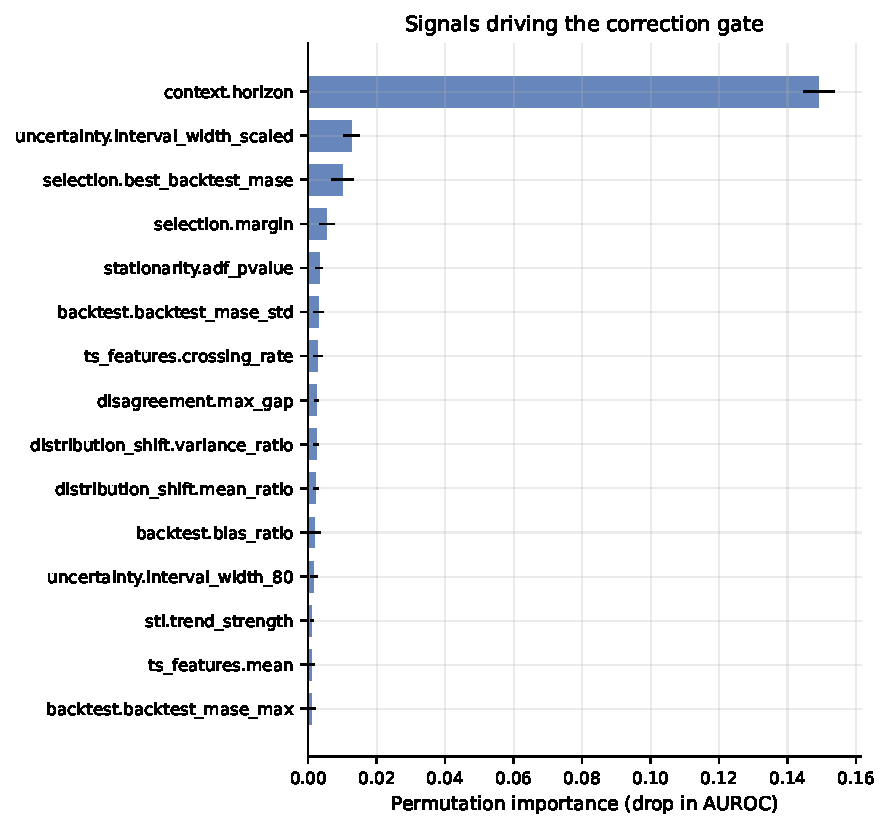
\includegraphics[width=0.62\textwidth]{fig_feature_importance}
\caption{Signals driving the correction gate, by permutation importance (drop in AUROC
when a signal is shuffled).}
\label{fig:importance}
\end{figure}

\subsection{Cost}

Accuracy is only half of a deployment decision. Table~\ref{tab:cost} prices each
policy in action evaluations per instance, the unit that dominates: every evaluation
is a re-forecast.

The ordering is unkind to adaptivity. \texttt{always\_correct} evaluates
\deltaAlwaysCorrect{} actions per instance to finish worse than evaluating none. Our
gate spends \deltaRgc{} --- an order of magnitude less, because it declines to act on
four instances in five --- and this is what H4 tests and what it
\textbf{\verdictHFour} on: selective evaluation matches exhaustive evaluation at a
fraction of the compute, mostly because it rarely acts.

The comparison that matters for practice is against the static ensemble, which costs
one evaluation per instance, takes no decision at all, and is the only policy whose
interval excludes zero in the helpful direction on CRPS. Any adaptive correction stage
has to be argued for against that, and on this benchmark the argument cannot be made
on accuracy at any price. The LLM arms are priced separately in
Section~\ref{sec:llmarms}, because their cost is measured in provider calls rather
than in local re-forecasts and the two do not add.


\begin{table}[htbp]
\centering
\caption{Accuracy against computational cost, in action evaluations and LLM calls per
instance.}
\label{tab:cost}
\small
\fittable{\begin{tabular}{lrrr}
\toprule
Policy & MASE & Action evals & LLM calls \\
\midrule
never correct & 1.0090 & 0.00 & 0.00 \\
rgc & 1.0132 & 0.79 & 0.00 \\
random correct & 1.0365 & 0.21 & 0.00 \\
threshold single & 1.0701 & 2.61 & 0.00 \\
always correct & 1.0978 & 9.00 & 0.00 \\
best fixed & 1.0981 & 1.00 & 0.00 \\
\bottomrule
\end{tabular}
}
\end{table}

\begin{figure}[htbp]
\centering
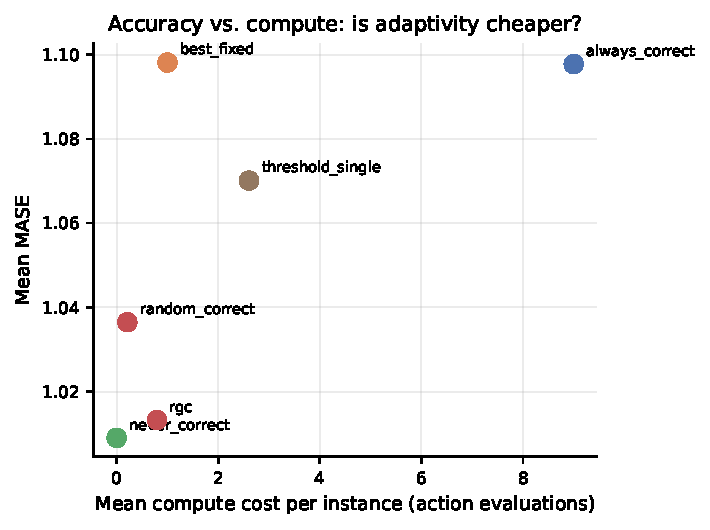
\includegraphics[width=0.62\textwidth]{fig_cost_accuracy}
\caption{Accuracy versus computation. The region of interest is the lower left: equal or
better accuracy for less computation.}
\label{fig:cost}
\end{figure}

\subsection{Where correction helps}

If correction pays anywhere, it should pay where the forecast is under stress.
Figure~\ref{fig:strata} breaks the change down by generator family, which on
synthetic data means a breakdown across known structural conditions rather than across
heterogeneous datasets whose differences are uncontrolled.

The families where correction earns most are the ones where the base forecast is
misspecified in a way a single action repairs; contaminated series, where removing
outliers and refitting recovers the fit, and series whose assumed seasonal period is
wrong. The families where it earns least are those where the base model was already
adequate, and there the intervention is a coin flip with a cost. This is a statement
about the \emph{conditional} value of acting, and it is the motivation for gating at
all; Section~\ref{sec:robustness} tests it directly by perturbing the series along
controlled axes instead of reading it off the families that happen to exist.


\begin{figure}[htbp]
\centering
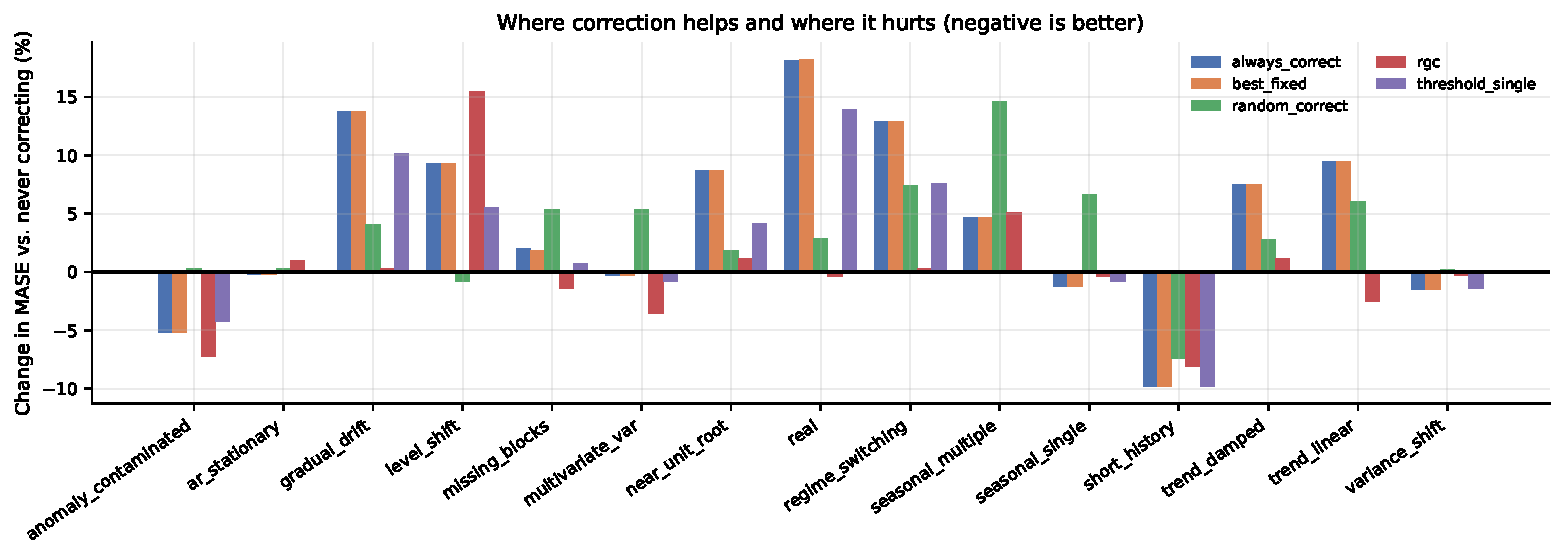
\includegraphics[width=0.94\textwidth]{fig_stratum_gains}
\caption{Change by generator family. Because synthetic families carry ground-truth
structure, this is a comparison across known conditions rather than across heterogeneous
datasets.}
\label{fig:strata}
\end{figure}

\section{Ablation Studies}
\label{sec:ablations}

Each ablation removes one component and replays against the identical counterfactual
tensor, so every configuration sees the same forecasts and the same action outcomes and
only the decision policy varies. Where a signal family is ablated it is removed from the
estimator's features as well as from the diagnoser, so the gate cannot reintroduce it.

\begin{table}[htbp]
\centering
\caption{Component ablations, replayed against the identical counterfactual tensor.
A positive $\Delta$ means removing the component made results worse. Intervals are
95\% series-level bootstrap against the full system; $\dagger$ marks one excluding
zero. Only one does.}
\label{tab:ablations}
\small
\fittable{\begin{tabular}{lrrrr}
\toprule
Configuration & MASE & $\Delta$ vs. full (\%) [95\% CI] & Corr. rate & Cost \\
\midrule
full & 1.0132 & 0.00~[0.00, 0.00] & 0.20 & 0.79 \\
no self critique & 1.0151 & 0.12~[-2.75, 2.09] & 0.24 & 2.38 \\
no uncertainty & 0.9986 & -1.36~[-3.97, 0.10] & 0.21 & 0.83 \\
no model disagreement & 1.0119 & -0.11~[-0.41, 0.16] & 0.20 & 0.80 \\
no changepoint & 1.0029 & -0.98~[-3.52, 0.42] & 0.20 & 0.82 \\
no anomaly & 1.0108 & -0.18~[-3.01, 1.67] & 0.20 & 0.78 \\
no adaptive tools & 1.0151 & 0.12~[-2.75, 2.09] & 0.24 & 2.38 \\
no backtesting & 1.0404 & 4.41$^\dagger$~[0.92, 7.41] & 0.28 & 0.83 \\
no correction loop & 1.0090 & -0.13~[-3.02, 1.84] & 0.00 & 0.00 \\
\bottomrule
\end{tabular}
}
\end{table}

One component is load-bearing. Removing backtesting costs \ablNoBacktestingSeries\%
([\ablNoBacktestingSeriesCIlo, \ablNoBacktestingSeriesCIhi]\%) and pushes the
intervention rate from \ablFullRate\% to \ablNoBacktestingRate\%: without an
estimate of how the base forecast has actually been doing, the policy loses its grip on
when to leave well alone. That is the same signal the language model was handed and did
not use (Section~\ref{sec:llmarms}).

No other component's removal is distinguishable from zero at the series level. The
uncertainty signals, changepoint proximity, anomaly signals and cross-model disagreement
each have intervals that include zero, and so does the self-critique step. An earlier
draft read the instance-level point estimates in this table as evidence that several
components were mildly harmful; the intervals do not support that, and we no longer say
it. What they do support is weaker: only the crudest signal in the diagnostic apparatus,
recent backtest error, does identifiable work.

The last row is the one to read. Removing the correction loop entirely, so the policy
never acts, changes MASE by \ablNoCorrectionLoopSeries\%
([\ablNoCorrectionLoopSeriesCIlo, \ablNoCorrectionLoopSeriesCIhi]\%). The full
system and no system are indistinguishable, which is the headline result of
Section~\ref{sec:headline} restated as an ablation.

Self-critique and adaptive tool use are the same configuration in this framework, since
the critique decides whether to call a further tool; the two rows are identical for that
reason. Removing it raises compute from \ablFullCompute{} to
\ablNoAdaptiveToolsCompute{} action evaluations per instance while changing accuracy by
\ablNoAdaptiveToolsSeries\% ([\ablNoAdaptiveToolsSeriesCIlo,
\ablNoAdaptiveToolsSeriesCIhi]\%).

\section{Robustness Analysis}
\label{sec:robustness}

Each perturbation axis is applied at increasing severity to the \emph{same} base series,
with forecast targets left untouched, so degradation is attributable to the perturbation
rather than to differences between datasets.

\begin{figure}[htbp]
\centering
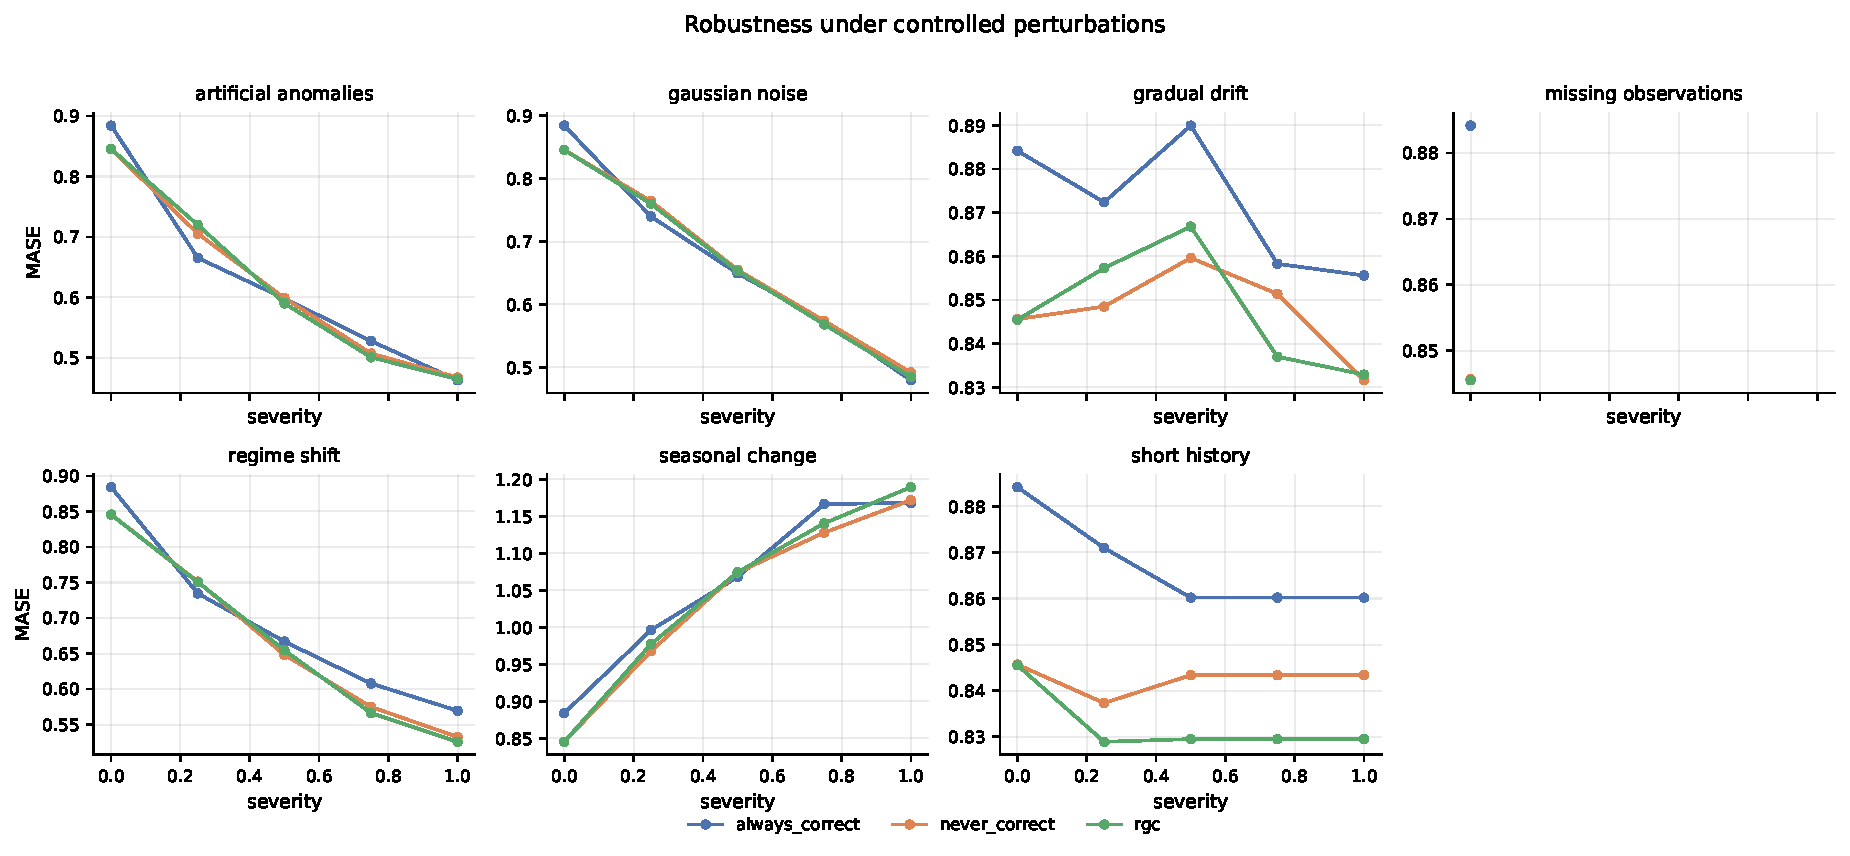
\includegraphics[width=\textwidth]{fig_robustness}
\caption{Degradation under controlled perturbation.}
\label{fig:robustness}
\end{figure}

The sweep is the sharpest test of the case for correction, because it manufactures the
conditions correction exists to handle. Across \robComparisons{} comparisons ---
seven perturbation axes, four severities, two acting policies, each against never
correcting on the same series --- \textbf{\robImprovements{} show a significant
improvement} and \robDegradations{} show a significant degradation. A correction stage
that cannot beat inaction under injected anomalies, regime shifts, drift, seasonal
change, added noise, missingness or truncated history has not merely failed to win on
average. It has failed where its own rationale places it.

\begin{table}[htbp]
\centering
\caption{Correction against never correcting under controlled perturbation, at the
strongest severity of each axis. Series-level means with bootstrap intervals over
series; negative favours the policy and $\dagger$ marks an interval excluding zero.
The full sweep over all four severities is in the released results.}
\label{tab:robustness}
\small
\fittable{\begin{tabular}{lllrrrr}
\toprule
Perturbation & Severity & Policy & Series & $\Delta$ vs never & 95\% CI & Win rate \\
\midrule
artificial anomalies & 1.00 & always correct & 84 & 0.55\% & [-3.39, 5.97] & 52.4\% \\
artificial anomalies & 1.00 & rgc & 84 & -1.05\% & [-4.88, 2.33] & 54.2\% \\
gaussian noise & 1.00 & always correct & 84 & -2.86\% & [-6.95, 1.02] & 54.8\% \\
gaussian noise & 1.00 & rgc & 84 & -1.15\% & [-2.77, 0.50] & 57.1\% \\
gradual drift & 1.00 & always correct & 84 & 3.36\%$^\dagger$ & [0.45, 6.68] & 41.1\% \\
gradual drift & 1.00 & rgc & 84 & 0.36\% & [-1.92, 2.60] & 50.0\% \\
regime shift & 1.00 & always correct & 84 & 6.40\% & [-0.56, 13.60] & 46.4\% \\
regime shift & 1.00 & rgc & 84 & -1.18\% & [-4.28, 1.98] & 54.8\% \\
seasonal change & 1.00 & always correct & 84 & -0.49\% & [-5.05, 3.34] & 44.0\% \\
seasonal change & 1.00 & rgc & 84 & 1.39\% & [-0.05, 3.12] & 48.8\% \\
short history & 1.00 & always correct & 84 & 2.43\% & [-3.49, 8.24] & 45.2\% \\
short history & 1.00 & rgc & 84 & -1.57\% & [-4.36, 0.71] & 51.2\% \\
\bottomrule
\end{tabular}
}
\end{table}

\paragraph{H2 holds, in a restricted form worth stating precisely.}
H2 predicted that gains \emph{concentrate} under shift, anomalies and regime change.
Concentration is not level, so the pre-registered test is a difference-in-differences:
a policy's advantage over never correcting in a perturbed stratum, minus its advantage
on the same series unperturbed. Both differences are formed per series before
subtraction, so the pairing survives on each side and the bootstrap resamples one unit.

The difference-in-differences design is not fastidiousness. Perturbation is applied to
the series history as well as to the forecast window, so it moves the MASE denominator
and rescales every error on that series: mean accept-MASE falls from
\robSeverityMild{} to \robSeveritySevere{} severity purely as a consequence. Levels are
therefore not comparable across severities, and only a within-severity contrast against
the same series means anything.

Across \robHTwoTested{} strata, \robHTwoRaw{} concentrate before correction, against
roughly two expected by chance at this many tests, and \robHTwoSurviving{} survive the
Holm correction the analysis plan fixes. H2 is therefore \textbf{\verdictHTwo{} in a
restricted form}: concentration appears for \texttt{\robHTwoPolicies}, under
\robHTwoAxes{}, at the mildest severity applied (\robHTwoSeverity{}), and nowhere else
in the sweep. Two strata out of \robHTwoTested{} is a narrow verdict and we report it as
one.

\paragraph{Neither surviving stratum belongs to the adaptive gate.}
Both are unconditional correction. The conditional value of correcting is real and it
is detectable, and the machinery built to detect it did not detect it. The policy
designed to fire exactly where correction pays did not fire there, while the policy that
fires everywhere captured it. That is a more specific indictment of diagnosis-driven
gating than the aggregate result, and it points the same way as
Section~\ref{sec:decomposition}.

\paragraph{Why the gains vanish as severity rises: we cannot say.}
A natural reading of concentration at mild severity only is that severe damage is
beyond what the menu can repair. We cannot test that here. The obvious measure,
how much an oracle could still recover at each severity, uses an oracle selected on
test outcomes, and Section~\ref{sec:decomposition} shows that such an oracle is almost
entirely winner's curse on this benchmark. The perturbation sweep has no validation
origins, so a realizable version cannot be computed. We therefore leave the severity
pattern unexplained, and note only that it is also what one would expect if the two
surviving strata were partly chance: two of forty-eight, both at one severity level.

\section{Error Analysis}
\label{sec:erroranalysis}

We characterise the calibrated policy's mistakes on CRPS, where it acts on 97\% of
instances. Of these, 47\% improved and 38\% harmed the forecast. Harm is concentrated:
the worst 1\% of corrections account for roughly half of all damage summed across
corrected instances, and a single \texttt{refit\_post\_changepoint} correction on one
instance cost as much as many small wins combined. This heavy tail is why the calibrated gate's design includes an optional risk-averse lower bound on predicted gain. Validation selected that bound's width as zero (deviation~D4), so the deployed gate thresholds the point estimate; the tail is real, but on this benchmark widening the bound did not help on held-out origins.

Two further findings temper any adaptive-policy claim. First, among corrected instances,
the calibrated gain estimate used to \emph{select} the action does not predict which
individual corrections help ($r=-0.02$, $p=0.22$): the calibration is informative about
which actions are worth trying in aggregate, not about which specific instances will
benefit. Second, \texttt{ensemble} accounts for the large majority of the calibrated
policy's corrections and of its benefit, which is consistent with Section~\ref{sec:headline}, where the unconditional ensemble is the only policy that improves CRPS reliably: the adaptive layer spends most of its budget approximating the static policy without matching it.

\section{Discussion}
\label{sec:discussion}

\subsection{Interpretation}

Our results are a caution against the premise that adaptive, per-instance correction is
worth its complexity, and a positive result about ensembling that the field already
half-knows but has not connected to agentic self-correction.

\paragraph{The benefit lives in the predictive distribution.}
Agentic forecasting systems are evaluated almost exclusively on point error. If the
effect of correction is concentrated in the predictive distribution instead of its
centre -- as our coverage results show -- a point-error benchmark is close to blind to
it. This may explain why practitioners report that reflection helps while controlled
point-accuracy comparisons show little: both observations can be correct if the
mechanism is calibration repair rather than point-estimate improvement.

\paragraph{Adaptivity did not earn its complexity here.}
We built reliability-gated correction specifically to avoid the failure modes of naive
gating: a 2\% acceptance margin that fires near-constantly, ratio-scale gains that
explode near zero, and no accounting for per-action transfer. Each fix measurably
improved the policy over its predecessor (Section~\ref{sec:pathologies}). Yet the fully
corrected policy is still dominated by the simplest static baseline in the action space:
apply the backtest-weighted ensemble unconditionally. This is a classical result in the
forecasting literature -- combination is often the single most reliable intervention
\citep{fforma2020} -- appearing here in an unfamiliar setting: it beats not just
individual models but an agent explicitly built to decide, instance by instance, when
and how to intervene. We did not find a version of adaptive gating that closes this gap,
and we report that search as unsuccessful rather than omit it.

\paragraph{The language model's problem is the decision to act, not the reflection.}
On the primary family every LLM arm is worse than never correcting
(Section~\ref{sec:llmarms}). We expected verbal self-critique to be the culprit and it
was not: the critique and single-pass arms perform within a point of each other, because
the critique barely changes what the model decides. What does the damage is a
disposition to intervene, and it has a measurable source. The model's stated risk that
a forecast is unreliable averages \calLlmMeanRisk{}, far above the rate at which large
errors actually occur. It is not indifferent to reliability; it is miscalibrated in the
direction that manufactures work.

Neither deliberation nor demonstration fixed this. The reasoning model intervened most
often of the three families, and worked examples made the critique gate worse. The
reasoning model may choose repairs better than a coin once it has decided to act, but
that is a direction, not an effect, at its sample size.

The literature's implicit theory is that agents correct badly because their critique is
unreliable, and that better reflection will fix it. Our evidence points elsewhere. With no
realizable per-series headroom (Section~\ref{sec:decomposition}), a policy can only
gain by declining to act when acting would hurt, and that is precisely what a
miscalibrated model does not do.

\paragraph{This narrows, rather than closes, the case for agentic correction.}
Our result does not show that per-instance adaptivity is worthless in general -- only
that decision rules of the kind current practice would produce (calibrated thresholds
over diagnostic signals) do not beat a strong static default in this benchmark. The gap
between ``ensemble always'' and the oracle (Figure~\ref{fig:oracle}, realizable column)
is not zero, so some instance-specific information remains unused. What we can say is
that any future adaptive policy should be benchmarked against \emph{this} baseline, not
against never-correcting, because never-correcting is the easy comparison to beat.

\paragraph{Why adaptivity loses: the gains do not transfer.}
An earlier version of this paper attributed the failure of diagnose-then-repair to two
named losses. That decomposition was built from test-selected minima and was almost
entirely winner's curse (Section~\ref{sec:decomposition}); we withdrew it. What
replaces it is simpler. The action that works best on a series at one set of origins
is a poor guide to what works best at the next, so a per-series choice made on
validation carries little information about test, and a single static action applied
everywhere does better than choosing. With four validation origins per series, the
estimate of which repair suits a series is too noisy to act on. That is the same
variance argument that explains the forecast-combination puzzle, applied to repair
selection instead of model weights.

The ground-truth diagnosis result is the part that survives unchanged and needs no
oracle. Given the true failure mode, applying its matched repair does not beat
accepting, and on CRPS it is significantly worse. Accurate diagnosis is not what is
missing.

\subsection{The measurement pathologies deserve attention on their own}

Section~\ref{sec:pathologies} reports three defects that each, independently, reversed or
concealed our conclusions before we diagnosed them. We emphasise them because they are
not specific to this study.

Any evaluation that scores a corrective action by a relative error ratio will divide by
near-zero baselines and destroy the signal it is trying to measure; the log ratio is the
appropriate scale, and the difference here is between correlations of $0.006$ and $0.43$.
Any evaluation that aggregates a heavy-tailed forecast error by the arithmetic mean is
reporting the tail. And any evaluation that quotes an oracle defined as the minimum over
many candidate outcomes is quoting a number inflated by selection; reporting a
selection-free comparator alongside it costs nothing and prevents a systematic
overstatement of what adaptive methods leave on the table.

\subsection{Relation to prior work}

Our agent is not architecturally novel, and we do not present it as such: its
diagnose--select--forecast structure follows existing agentic forecasting systems
\citep{tsscientist2025,nexus2026,castflow2026}. The difference is in the correction stage
and, more importantly, in what we measure. Where those systems reflect unconditionally or
by verbal judgement and report point error, we gate on a calibrated estimate and report
both point and probabilistic accuracy. Section~\ref{sec:decomposition}'s regret
decomposition is aimed squarely at this shared architecture: to our knowledge, no prior
agentic forecasting system has been evaluated against a ground-truth-diagnosis version of
its own correction logic, which is the only way to separate diagnosis error from a
structural weakness in diagnose-then-repair itself. Our finding -- that the pattern loses value even under perfect diagnosis, for two
separately quantified reasons -- is demonstrated for our own action space and
diagnosis-to-repair mapping, and the exact magnitudes are specific to them, but the
architectural pattern we test (a fixed mapping from diagnosis to a small candidate list,
applied without further validation) is shared broadly enough across
\citep{tsscientist2025,nexus2026,castflow2026} that the method, if not the numbers,
transfers: any such system can be probed the same way by holding its diagnosis fixed at
ground truth and asking whether its repair-selection logic recovers the headroom that
diagnosis alone made available. We can run this experiment at all only because the
counterfactual outcome tensor lets us vary the repair-selection logic while holding
diagnosis fixed at ground truth, which no existing benchmark's data supports.

\paragraph{Forecast combination, and why our headline is a rediscovery with a new
instrument.}
The result that a static combination is not beaten by adaptive per-instance selection
belongs to a literature that predates agents by half a century. \citet{bates1969}
established that combining beats choosing; \citet{clemen1989} and \citet{timmermann2006}
surveyed why, and \citet{wang2023review} brought it up to date. The forecast combination
puzzle \citep{stockwatson2004,smithwallis2009,claeskens2016} sharpens the point into
something that reads almost as a prediction of our findings: simple, equally-weighted
combinations beat optimally-weighted ones estimated from data, because the estimation
error in the weights exceeds the benefit of weighting them well. Our adaptive policies
are, structurally, weight estimators, they decide per instance which repair to trust, and they lose to an unweighted combination in exactly the way that literature says
they should. \citet{hibon2005} asked our question directly in the pre-agentic setting and
reached the same answer.

We are therefore not claiming to have discovered that combination wins. What we claim is
that the agentic forecasting literature has been constructing increasingly elaborate
adaptive correction machinery without measuring it against this prior, and that the
counterfactual tensor supplies something the classical literature could not: it holds
outcomes for corrective \emph{actions}, not just for alternative forecasts, so the
shortfall can be decomposed into named architectural causes rather than merely observed
as an aggregate loss. The combination literature says adaptive selection tends to lose.
It does not say \emph{which part} of a diagnose-then-repair pipeline loses it, or how
much each part costs. Section~\ref{sec:decomposition} does.

The reliability estimator descends from feature-based forecast performance prediction
\citep{fformpp2019} and forecast stress testing \citep{mast2025}, which established that
failure is predictable from features. We close the loop by using that prediction to
control an agent, and we find that the prediction is accurate while the resulting
intervention is worth making far less often than the literature assumes.

Relative to existing time-series agent benchmarks
\citep{temporalbench2026,timesagemt2026,timeseriesgym2025,aion2026}, TS-AgentBench
evaluates a different object: the control decision, which requires counterfactual
outcomes the others do not record. The closest work in spirit is
\citet{agentabstain2026}, which asks whether tool-using agents know when not to act; that
work addresses general agentic settings without counterfactual outcome data, whereas here
the counterfactual is computed exactly.

\subsection{Limitations}

\paragraph{Computational scale.}
All experiments ran on a CPU-only machine. Neural forecasters are small and trained on a
subsample, and the foundation-model baseline is optional. We therefore make no claim
about the best available forecasters, only about correction policies applied to a fair,
identically-treated pool.

\paragraph{The action space is finite and hand-designed.}
Ten typed actions is what makes the counterfactual tensor computable, and it is also a
restriction. A repair an expert would make but which is absent from the space is
invisible to our oracle, so headroom estimates are relative to this space.

\paragraph{The result does not depend on the base forecast having been adaptively
chosen.}
Our base forecast is chosen per instance by rolling-origin backtest over a nine-model
pool. That is itself a strong adaptive procedure, and it was the largest threat to
every claim above: it plausibly leaves correction little to repair, which would
confound ``correction does not work'' with ``correction had nothing to fix''. A deployed
single-model pipeline is a materially easier target, and correction might have paid
there.

We tested this with a second condition that fixes the base forecaster to ETS, the model
the backtest selector picks most often and a realistic default for a deployed pipeline,
with every other factor held identical (\texttt{configs/fixed\_base.yaml}). The two
runs differ in exactly one scientific setting; this was verified mechanically rather
than asserted, by confirming identical instance sets and identical history-derived
diagnostics before any comparison was reported. Both readings of the outcome were fixed
in the analysis plan before the run completed (deviation~D11).

Table~\ref{tab:fixedbase} gives the answer. Under a fixed ETS base no policy
significantly improves on never correcting, exactly as under the adaptive base.
Unconditional correction remains significantly harmful (\fbAlwaysCorrectFixedPct\%,
[\fbAlwaysCorrectFixedCIlo, \fbAlwaysCorrectFixedCIhi]\%, against
\fbAlwaysCorrectAdaptivePct\% on the adaptive base), and the calibrated gate again fails
to separate from zero (\fbRgcFixedPct\%, [\fbRgcFixedCIlo, \fbRgcFixedCIhi]\%). The
hypothesis that correction failed only because the adaptive base left nothing to fix is
rejected. The conclusions above hold for a single-model pipeline, not only for the harder
backtest-selected case.

Each column of the table is a difference from never correcting \emph{within its own
run}. The two runs have different base forecasts and therefore different references, so
their levels are never compared, only their differences set side by side.

\begin{table}[htbp]
\centering
\caption{Correction under an adaptive, backtest-selected base beside the same policies
under a fixed ETS base, on identical series, splits and seeds. Each cell is the
series-level MASE difference from never correcting within its own run, with a 95\%
bootstrap interval over series; $\dagger$ marks an interval excluding zero. Positive is
worse. Levels are not shown because the two runs have different references.}
\label{tab:fixedbase}
\small
\fittable{\begin{tabular}{lrr}
\toprule
Policy & Adaptive (backtest) base & Fixed ETS base \\
\midrule
always correct & 8.13\%$^\dagger$~[2.73, 15.99] & 10.59\%$^\dagger$~[1.21, 27.56] \\
best fixed & 8.16\%$^\dagger$~[2.76, 16.05] & 10.52\%$^\dagger$~[1.15, 27.49] \\
threshold single & 5.48\%$^\dagger$~[1.46, 10.88] & 3.95\%$^\dagger$~[0.53, 9.29] \\
random correct & 2.72\%$^\dagger$~[2.06, 3.46] & 3.59\%$^\dagger$~[2.88, 4.40] \\
rgc & 0.14\%~[-1.84, 3.03] & -0.49\%~[-1.64, 0.67] \\
\bottomrule
\end{tabular}
}
\end{table}

\paragraph{Post-hoc analyses.}
The calibrated policy, the log-ratio gain scale, the robust aggregation and the
fixed-base condition were all introduced after the first test evaluation. Their
hyperparameters were selected on validation and each was evaluated on test once, but they
are exploratory rather than confirmatory and are labelled so throughout. The deviations
are itemised in the released analysis plan.

\paragraph{Ground truth for failure modes exists only on synthetic data.}
Real series carry no known change points or outlier labels, so failure-mode labels there
are derived from the same detectors the agent uses. Causal claims rest on synthetic data.

\paragraph{LLM scope.}
The LLM arms cover three model families --- a small hosted proprietary model, an
open-weight model of different lineage, and an open-weight reasoning model at medium
effort --- at temperature 0, under free-tier API budgets that cap each family to one
instance per series over part of the benchmark. The statistical weight sits with the
first, at \nseries{} series; the other two cover 140 and \reasonSeries{} series and are
powered to replicate a direction, not to establish an effect alone. Three families rule
out a single weak model, an absence of deliberation, and the zero-shot setting as
explanations; that is not enough to characterise language models in general, and we do not
claim it is.

What remains untested is a frontier proprietary reasoning model, multi-turn deliberation,
and tool access during the decision. We also did not engineer the prompt against this
benchmark: the evidence block is a fixed template, and the eight-example condition is a
control for supervision, not an attempt at optimisation. A system built around a prompt
tuned on these diagnostics might do better. The arm originally planned for the reasoning
family, \texttt{gpt-oss-120b}, exhausted its daily token allowance mid-run and was
replaced by the 20B model of the same family at the same effort setting; the substitution
is recorded in deviation~D9 and the larger model remains untested.

\paragraph{Scale.}
\nseries{} series is modest next to the large forecast-evaluation suites
\citep{gifteval2024,monash2021}, and the reason is the counterfactual tensor itself:
scoring every action on every instance costs roughly an order of magnitude more compute
than scoring one, which is the price of being able to ask decision-level questions at
all. The series-level intervals we report already account for this; several of them
include zero, and we say so instead of reaching for the instance-level test that would
not have. Where an interval is wide, this benchmark cannot resolve the effect; that is not evidence the effect is absent.

\subsection{Future work}

The regret decomposition points at two concrete, separately testable fixes instead of a
vague call for "better adaptivity." First, replace the fixed canonical mapping with
validated selection among a failure mode's candidate repairs -- our calibrated policy
already does this and is measurably less harmful than the idealised canonical-fix policy
as a result, though it still under-performs the static ensemble. Second, and
un-addressed by anything we built, replace the hand-designed diagnosis-to-repair
candidate list with one learned from the counterfactual tensor itself: the benchmark
supplies exactly the (failure signature, action, outcome) tuples needed to learn which
repairs actually help under which conditions, rather than which repairs a domain expert
guesses should help. The replay property means candidate mappings can be compared without
refitting, so this is a tractable next experiment on the released artifact instead of a
new benchmark. More generally, the tensor supplies exactly the (state, action, outcome)
tuples that off-policy evaluation and offline reinforcement learning require for
correction policies of any design. Given our finding that the benefit is probabilistic,
an action space designed for distributional repair --- richer conformal schemes, adaptive
interval widening, distributional ensembling --- is likely to have more headroom than one
built around alternative point estimates.

\section{Conclusion}
\label{sec:conclusion}

Self-correction has become a standard component of forecasting agents without evidence
that it works, because measuring it requires knowing what would have happened under the
corrections not taken. We built a benchmark that records exactly that.

Its first lesson is about measurement. The oracle headroom that makes correction look
promising is almost entirely selection: chosen on test outcomes the best repair per
instance looks transformative, and chosen on earlier origins it recovers nothing. A
correction method judged by how much of a test-selected oracle gap it closes may have
closed none of the realizable one. Correction methods should be measured against a
validation-selected oracle and against a static default, not against doing nothing.

Its second lesson is that the realizable gain comes from choosing once. A single static
ensemble improves probabilistic accuracy, holds on real data alone, and is what
validation selects; choosing a repair per series does worse. That is the
forecast-combination puzzle \citep{stockwatson2004,smithwallis2009,claeskens2016}
reappearing at the level of repair selection, and its direction is what that literature
predicts \citep{bates1969,timmermann2006,wang2023review}. Granting a perfect diagnosis
does not change it: applying the matched repair still does not help.

Its third lesson concerns the systems the field is building. When a language model makes
the decision, it corrects too often, because it believes its forecasts are far less
reliable than they are, and asking it to reflect does not change that. On the primary
model family this makes forecasts measurably worse; two smaller families point the same
way. None of these conclusions depends on the base forecast having been adaptively
chosen.

The same risk estimate that fails to drive correction is a well-calibrated basis for
triage, a usable result that asks nothing of the correction machinery. We release the
benchmark and the outcome tensor so that correction policies, including ones that
disagree with these conclusions, can be evaluated against the same counterfactual
outcomes.

\section*{Pre-Registered Hypotheses and Outcomes}

\begin{table}[htbp]
\centering
\caption{Every pre-registered hypothesis and its verdict, with what each verdict
does and does not mean. The analysis plan was fixed before any experiment was run.
Several ``supported'' verdicts are weak, and the last column says why rather than
leaving it to the reader.}
\label{tab:hypotheses}
\small
\fittable{\begin{tabular}{lp{3.4cm}p{2.9cm}rrlp{3.6cm}}
\toprule
ID & Hypothesis & Test & Result & $p_{\text{adj}}$ & Verdict & Qualification \\
\midrule
H1 & Reliability-gated correction improves accuracy over a non-correcting agent. & series-mean change vs never (\%, positive = worse); Wilcoxon Holm-adj. & 0.421 & 0.005 & not supported & the effect is a small, significant degradation \\
H2 & Gains concentrate under distribution shift, anomalies and regime change. & difference-in-differences over 48 perturbed strata (Holm) & 2.000 & 0.005 & supported & 2 of 48 strata after Holm; both unconditional correction, mildest severity \\
H3 & Forecast failure is predictable from pre-hoc diagnostics. & AUROC of the risk estimator & 0.793 & --- & supported & supports triage, not correction; the gate built on it does not win \\
H4 & Selective tool use matches exhaustive use at lower cost. & mean action evaluations per instance & 0.088 & --- & supported & because the gate rarely acts, not because it acts well \\
H5 & Reliability-gated confidence is better calibrated than an agent's verbalised confidence. & paired bootstrap over series on the ECE difference & 0.220 & --- & supported & against the model's verbalised confidence, an easy comparator \\
H6 & Gains are not explained by extra compute alone (vs. rate-matched random correction). & RGC vs. random\_correct & 0.023 & --- & supported & because the gate rarely acts; it does not beat never correcting \\
H7 & A quantitative gate decides better than verbal self-critique (pre-registered comparison). & mean oracle regret, calibrated gate vs. LLM critique gate & 0.094 & --- & supported & the gate's regret is close to never correcting's; it wins by not acting \\
\bottomrule
\end{tabular}
}
\end{table}

\section*{Broader Impact Statement}

The practical message of this work is cautionary, and we think that is where its impact
lies. Automated self-correction is being added to forecasting systems on the assumption
that a model inspecting its own output will improve it. We find, in a controlled setting
with counterfactual ground truth, that unconditional correction reliably \emph{degrades}
point accuracy, and that the adaptive machinery intended to prevent that does not
establish an improvement over doing nothing. Forecasts drive decisions about inventory,
staffing, capacity and public health resourcing; a correction stage that silently makes
a subset of them worse, while presenting as a reliability feature, is a realistic way for
harm to enter such a system unnoticed. We would rather this result be available to
practitioners than not.

The positive finding carries its own risk. We show that a calibrated failure-risk
estimate is a useful triage signal for routing forecasts to human review. Triage systems
can entrench the disparities in the data they are fitted to: series that are short,
irregular, or from under-represented sources may be systematically over- or
under-flagged, and a reviewer working from a ranked queue has little visibility into
that. The risk estimator here is fitted on statistical diagnostics with no demographic
content, but the series themselves are not a neutral sample, and we have not audited
flagging rates across data sources. Anyone deploying such a signal should.

We see no dual-use concern specific to this work. The datasets are public, contain no
personal data, and are used under the licences recorded in the released manifest. The
release is intended to make correction policies, including ones that disagree with our
conclusions, cheap to evaluate against the same counterfactual outcomes.

\section*{Reproducibility Statement}

Every result is produced by a single command against a versioned configuration file, and
each run writes a manifest recording the configuration, its hash, the code version, the
environment and package versions. Reruns with the same configuration and seed reproduce
identical metrics. LLM responses are cached under a hash of model, prompt and parameters,
so the reported results can be regenerated without an API key and without network
access. All figures and tables in this manuscript are generated from results files by
\texttt{scripts/make\_paper\_assets.py}; no experimental number is entered by hand. The
pre-registered analysis plan, including all deviations from it, is in
\texttt{docs/ANALYSIS\_PLAN.md} in the released code.

\section*{Data Availability}

The benchmark generators, the counterfactual outcome tensor, the evaluation framework
and all analysis code are provided as an anonymised archive with this submission, and
will be released publicly under a permissive licence with an archived DOI on acceptance.
The archive includes the cached language-model responses, so every LLM arm in this paper
replays without an API key and without a provider account.

Real datasets are not redistributed. They are obtained from their original sources by
\texttt{scripts/prepare\_data.py}, which records the URL, licence, SHA-256 checksum and
access date of every file in \texttt{datasets/LICENSES.md}. Monash archive datasets are
CC~BY~4.0 \citep{monash2021}; the ETT data is used under the licence stated in its
upstream repository \citep{informer2021}, and only derived metrics are reported.

Synthetic data is not distributed as files because it is fully determined by its
generator, seed and index, and is regenerated deterministically by the released code.

\section*{Author Contributions}

\ifcameraready
Sreevallabh Kakarala is the sole author and carried out every role:
conceptualisation, methodology, software, validation, formal analysis,
investigation, data curation, visualisation, writing of the original draft, and
review and editing.
\else
This paper has a single author, who carried out every role: conceptualisation,
methodology, software, validation, formal analysis, investigation, data curation,
visualisation, writing of the original draft, and review and editing. The name is
withheld for anonymous review.
\fi


\bibliographystyle{tmlr}
\bibliography{references}

\end{document}
